\documentclass[oneside,12pt]{Classes/aesm_edspia}

% Unicode and Arabic support
\usepackage[T1]{fontenc}
\usepackage[utf8]{inputenc}
\usepackage[arabic,french,english]{babel}
% \usepackage{arabtex}
\usepackage{epstopdf}

\usepackage{amsmath}
\usepackage{lmodern}%font modern
\rmfamily
\DeclareFontShape{T1}{lmr}{bx}{sc}{<->ssub * cmr/bx/sc}{} 
\usepackage{lettrine}
\usepackage{tabularx}
\usepackage{epsfig, floatflt, amssymb} 
\usepackage{moreverb} %% pour le verbatim en boite
\usepackage{cases}%equations en systemes numérotés - soluce possible package : CASES
\usepackage{multirow} %% pour regrouper un texte sur plusieurs lignes dans une table
\usepackage{url} %% pour citer les url par \url
\usepackage[all]{xy} %% pour la barre au dessus des symboles
\usepackage{textcomp} %% pour le symbol pour mille par \textperthousand et degrés par \degres
\usepackage[right]{eurosym}
\usepackage{setspace} %interligne simple, double etc...
\usepackage{Classes/eurosans} %%pour le symbole \euro
\usepackage{epic,eepic}
\usepackage{soul}
\usepackage[nottoc]{tocbibind} % tables des figures, des matieres et autres dans la TOC
\usepackage{fancybox}
\usepackage[leftcaption]{sidecap}
\usepackage[labelsep=endash, textfont={footnotesize, singlespacing}, margin=10pt, format=plain, labelfont=bf]{caption}
\usepackage[Conny]{Classes/fncychap} %en tete chapitrage
\newcommand{\ie}{c.-\`a-d.~}
\hbadness=10000% pb d'overfull box réglé
\hfuzz=50pt
\pdfcompresslevel9 % pour compresser le pdf final au maximum
\pdfoptionpdfminorversion=5 % pour accepté les images PDF version 1.5 (ex: celles produites par Office 2007)
\def\underscore{\char`\_}
\makeatletter
\renewcommand{\thesection}{\arabic {section}}
\renewcommand{\SC@figure@vpos}{c}% centrer verticalement le caption avec le package sidecap...
\renewcommand{\fnum@figure}{\small\textbf{Figure~\thefigure}}
\renewcommand{\fnum@table}{\small\textbf{Table~\thetable}}

\makeatother
\usepackage{subfig}
\usepackage{pdflscape} % for landscape pages
\usepackage{pgfgantt} % for Gantt charts
\def\thechapter{\Roman{chapter}}

%\usepackage[framed,numbered,autolinebreaks,useliterate]{Classes/mcode}


%%% Listings

\usepackage{listings}
\lstloadlanguages{xml, java}
	
  \usepackage{courier}
 \lstset{
         basicstyle=\footnotesize\ttfamily, 
         %numbers=left,               
         numberstyle=\tiny,          
         %stepnumber=2,               
         numbersep=5pt,              
         tabsize=2,                  
         extendedchars=true,         
         breaklines=true,            
         keywordstyle=\color[rgb]{0.43,0,0}\textbf,
        frame=b,
         commentstyle=\color[rgb]{0.51,0.51,0.51} \textit ,
         stringstyle=\ttfamily  \color[rgb]{0,0.44,0} ,
         showspaces=false,           
         showtabs=false,             
         xleftmargin=17pt,
         framexleftmargin=17pt,
         framexrightmargin=5pt,
         framexbottommargin=4pt,
         %backgroundcolor=\color{lightgray},
         showstringspaces=false            
 }
 
\DeclareCaptionFont{white}{\color{white}}
\DeclareCaptionFont{red}{\color{red}}
\DeclareCaptionFont{black}{\color{black}}
\DeclareCaptionFormat{listing}{\colorbox[cmyk]{0.43, 0.35, 0.35,0.01}{\parbox{\textwidth}{\hspace{15pt}#1#2#3}}}
\captionsetup[lstlisting]{format=listing,labelfont=black,textfont=white, singlelinecheck=false, margin=0pt, font={bf,footnotesize}}


%%%%%%%%%%%%%%%%%%%%%%%%%%%%%%%%%%%%%%%%%%%
\begin{document}
%%%%%%%%%%%%%%%%%%%%%%%%%%%%%%%%%%%%%%%%%%%
\hypersetup{pageanchor=false}
\hypersetup{backref=false,pagebackref=false}
\renewcommand\figurename{\small\textbf{Figure}} 

\addtocounter{page}{-1}%pour revenir à 0

% Pour remplir la page de garde

\TitreProjet{Enforcing Best Practices with LLM-IDE Integration}

\AuteurA{Arij} {KOUKI} 
\HostedBy{
\includegraphics[width=0.3\textwidth]{Images/google_logo.png}}


\Encadrant{Ms.}{Rabaa}{YOUSSEF}
\EncadrantS{Ms.} {Irene} {LOPEZ}

\Filiere{Software Engineering}
\datesout{30/09/2025}



\President{Ms. President} {Ghada GASMI}     %% Président du Jury
\RapporteurA{Ms. Reviewer} {Asma BEN HASSOUNA} %%Rapporteur



\AnneeUniv{2024/2025}
%%%%%%%%%%%%%%%%%%%%%%%%%%%%%%%%%%%%%%%%%%%
\makethese %% crée la couverture.
\makesecond
\hypersetup{pageanchor=true}

\onehalfspacing

% une page blanche (deuxième de couverture)
\newpage\thispagestyle{empty}\addtocounter{page}{-3}
\null\newpage\thispagestyle{empty}


\frontmatter %numérotation en iii
\pagestyle{fancy}
\fancyhf{}
\fancyhead[R]{Remerciements}
\fancyfoot[R]{\thepage}
\renewcommand{\headrulewidth}{0.5pt}
\renewcommand{\footrulewidth}{0pt}

\chapter*{Acknowledgements}
%===================================================================

I wish to extend my deepest gratitude and appreciation to everyone who has contributed significantly to the successful completion of this project.

My sincere thanks go to Irene Lopez and Andrew Xue, my host and co-host at Google Zurich, for their invaluable guidance, support, and trust throughout my internship. Their mentorship and kindness made this experience not only enriching but truly transformative.

Thank you to the YouTube Developer Infrastructure team for their warm welcome, collaborative spirit, and continuous encouragement, and to my mentor Veronica Radu, whose insights and support greatly contributed to my personal and professional growth.

I also wish to thank Mrs. Rabaa Youssef, my academic supervisor, for accompanying me in this final academic milestone.

To the distinguished members of the jury, I am grateful for your time and consideration in reviewing my work. I hope this report lives up to the standards expected of a graduation project.

To the professors of the National Institute of Applied Sciences and Technology, thank you for playing a vital role in shaping my academic and professional foundation.

And to my family and friends, your unwavering belief in me has carried me through the most demanding moments. Thank you for your love, patience, and presence.

Finally, a quiet note of gratitude to myself for the perseverance and dedication that made this journey possible.

%%%%%%%% Abstract/Resume
\fancyhead[R]{Abstract}
\chapter*{Résumé}
\addcontentsline{toc}{chapter}{Résumé}
%===================================================================

Ce projet a été réalisé chez Google Zurich dans le cadre d’un Diplôme National d’Ingénieur en Génie Logiciel. Il explore l’intégration de l’intelligence artificielle générative dans le processus de développement logiciel en incorporant un agent basé sur un Large Language Model (LLM) au sein d’un Environnement de Développement Intégré (IDE) interne.

Cet agent effectue une analyse approfondie du code afin de détecter des violations complexes ou subjectives que les outils d’analyse statique traditionnels peuvent négliger. En générant des explications claires et compréhensibles ainsi que des suggestions concrètes, il aide les développeurs, notamment ceux contribuant à YouTube, à maintenir une haute qualité de code et à respecter les bonnes pratiques. Intégré de manière transparente au sein du flux de travail via une extension de l’IDE, l’agent améliore la productivité et contribue à la réduction de la dette technique sans perturber l’expérience de développement.

Ce travail met en évidence le potentiel des outils assistés par l’IA pour transformer l’expérience des développeurs et ouvre des perspectives pour l’avenir des environnements de développement intelligents.\\

\textbf{Mots-clés : Intelligence Artificielle Générative, Génie Logiciel, Intégration IDE, Qualité du Code, Productivité des Développeurs}

\chapter*{Abstract}
\addcontentsline{toc}{chapter}{Abstract}
%===================================================================

This project was carried out at Google Zurich as part of a National Engineering Diploma in Software Engineering. It investigates the integration of generative artificial intelligence into the software development process by embedding a Large Language Model (LLM)-powered agent within an internal Integrated Development Environment (IDE).

The agent performs in-depth code analysis to detect complex or subjective violations that traditional static analysis tools may overlook. By generating clear, human-readable explanations and actionable suggestions, it supports developers, particularly those contributing to YouTube, in maintaining high code quality and adhering to best practices. Seamlessly integrated into the development workflow through an IDE extension, the agent enhances productivity and helps reduce technical debt without disrupting the coding experience.

This work demonstrates the potential of AI-assisted tooling to transform the developer experience and raises broader implications for the future of intelligent software engineering environments.\\

\textbf{Keywords: Generative AI, Software Engineering, IDE Integration, Code Quality, Developer Productivity}




%%%%%%%% TOC

%profondeur dans la table des matières et de la numérotation des sections

\setcounter{secnumdepth}{3}
\setcounter{tocdepth}{3}


\renewcommand{\contentsname}%
    {Table of Contents}%

%%%%minitoc
%\dominitoc % génère la minitoc
%\nomtcrule % supprime les lignes horizontales de la minitoc
%\renewcommand{\mtctitle}{Summary} % Modifie le titre de la minitoc

%%%%
\tableofcontents

\renewcommand{\headrulewidth}{0.5pt}
\renewcommand{\footrulewidth}{0pt}
\fancyhead[R]{Table des Matières}


%%%%%%%% Figures

\makeatletter
%\renewcommand{a\thefigure}{\@arabic\c@figure}
\@addtoreset{figure}{chapter}
\makeatother

\renewcommand{\headrulewidth}{0.5pt}
\renewcommand{\footrulewidth}{0pt}
\renewcommand\listfigurename{List of Figures}

\listoffigures 

\fancyhead[R]{List of Figures}
\newpage


%%%%%%%% Tableaux

\makeatletter

\renewcommand{\headrulewidth}{0.5pt}
\renewcommand{\footrulewidth}{0pt}
\renewcommand\listtablename{List of Tables}

\listoftables 

\fancyhead[R]{List of Tables}
%%%%%%%% Acronyms
\fancyhead[R]{List of Acronyms}
\chapter*{List of Acronyms}
\addcontentsline{toc}{chapter}{List of Acronyms}

\begin{spacing}{1.2}

\begin{table}[H]
\centering
\begin{tabular}{p{3cm}p{12cm}}
\textbf{AI} & Artificial Intelligence \\
\textbf{API} & Application Programming Interface \\
\textbf{CI/CD} & Continuous Integration/Continuous Deployment \\
\textbf{DL} & Deep Learning \\
\textbf{FIFO} & First In, First Out \\
\textbf{IDE} & Integrated Development Environment \\
\textbf{JSON} & JavaScript Object Notation \\
\textbf{LLM} & Large Language Model \\
\textbf{ML} & Machine Learning \\
\textbf{QA} & Quality Assurance \\
\textbf{RPC} & Remote Procedure Call \\
\textbf{SDLC} & Software Development Life Cycle \\
\textbf{VS} & Visual Studio \\
\end{tabular}
\end{table}

\end{spacing}


%%%%%%%%%%%%%%%%%%%%%%%%%%%%%%%%%%%
                     
\mainmatter %numéros arabes
\pagestyle{fancy}
\fancyhead[R]{Introduction Générale}
\chapter*{General Introduction}

\addcontentsline{toc}{chapter}{General Introduction}
\begin{spacing}{1.2}
%==================================================================================================%

The software engineering industry is experiencing a major shift driven by the rapid evolution of artificial intelligence and the growing demand for scalable, high-quality code development practices. As development teams grow and systems become more complex, ensuring consistent code quality and adherence to best practices presents an ongoing challenge, especially in large organizations managing massive codebases across distributed teams.\\

Traditional static analysis tools and linters, while helpful, often fall short when it comes to identifying nuanced or subjective coding issues that depend on context or internal guidelines. In fast-paced development environments, engineers need intelligent, responsive tools that go beyond rule-based checks to provide deeper insights and real-time guidance, without adding friction to their daily workflows.\\

This graduation project explores the integration of generative artificial intelligence into modern Integrated Development Environments (IDEs) to support software engineers in their day-to-day coding activities. The research investigates how Large Language Models (LLMs) can be leveraged to perform in-depth code analysis, detect complex violations, and offer clear, contextual suggestions for improvement. By embedding intelligent assistance directly within the development workflow, this work aims to enhance code quality, reduce technical debt, and support developer productivity at scale.\\

This report begins by establishing the theoretical foundation and examining the current state of AI-assisted development tools. It then presents the design and implementation of an intelligent code analysis system, followed by an evaluation of its effectiveness in real-world development scenarios. The work contributes to the broader understanding of how artificial intelligence can transform software engineering practices and improve developer experience.




\end{spacing}



\fancyhf{}
\fancyhead[R]{Introduction Générale}
\fancyfoot[R]{\thepage}
\renewcommand{\headrulewidth}{0.5pt}
\renewcommand{\footrulewidth}{0pt}


\setcounter{mtc}{5} %indique le numéro réel du chapitre, pour la mini table des matières
\chapter{Project Overview}
\minitoc  %insert la minitoc

\graphicspath{{Chapitre1/figures/}}
%==============================================================================
\pagestyle{fancy}
\fancyhf{}
\fancyhead[R]{\bfseries\chaptername~\thechapter. }
\fancyfoot[R]{\thepage}
\renewcommand{\headrulewidth}{0.5pt}
\renewcommand{\footrulewidth}{0pt}
%\renewcommand{\chaptermark}[1]{\markright{\MakeUppercase{\chaptername~\thechapter. #1 }}{}}
%\renewcommand{\sectionmark}[1]{\markright{\thechapter.\thesection~ #1}}

\begin{spacing}{1.2}
%==============================================================================

\section*{Introduction}
This opening chapter establishes the foundation of the graduation project by introducing the
host company and defining the project’s scope. We examine the organizational context,
outline the main objectives and challenges, and present the methodological framework that
guides the development process.


\section{Host Company: Google} 

\subsection{Presentation} 
Founded in 1998, Google LLC is a global leader in technology and innovation. As a subsidiary of Alphabet Inc., Google’s mission is to organize the world’s information and make it universally accessible and useful. Guided by values such as innovation, accessibility, sustainability, and user trust, Google has established itself as one of the most influential companies shaping the digital era. Its culture emphasizes collaboration, diversity, inclusion, and impact-driven engineering, enabling continuous leadership in research and product development.

\begin{figure}[!ht]\centering

\includegraphics[scale=0.06]{Images/google_logo.png}
\caption{Google Logo}
\label{fig:google_logo}
\end{figure}

\subsection{Products and services} 
Google offers a broad ecosystem of products and services that touch nearly every aspect of digital life. Among its flagship consumer products are Google Search, Maps, Gmail, Chrome, and the Android operating system, serving billions of users daily. 

Beyond consumer services, Google develops enterprise and cloud-based solutions such as Google Cloud Platform and Google Workspace, as well as advanced AI systems like Vertex AI. The company also invests in hardware, including Pixel devices, Nest smart home products, and ChromeOS. 

These products reflect Google’s commitment to connecting people, improving productivity, and driving digital transformation worldwide.

\begin{figure}[!ht]\centering
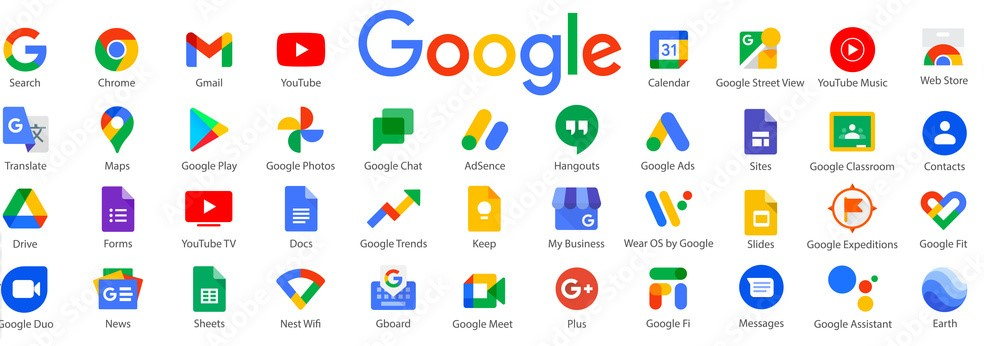
\includegraphics[scale=1.1]{Images/google_products.jpg}
\caption{Overview of some Google products}
\label{fig:google_products}
\end{figure}

\subsection{Focus Area} 
\subsubsection{YouTube}
Acquired by Google in 2006, YouTube has become the world’s leading video-sharing platform, serving more than two billion logged-in users monthly. It empowers individuals to create, share, and discover video content globally while sustaining a vibrant creator economy. From a technical perspective, YouTube integrates video processing, recommendation systems, live streaming, advertising, and trust and safety to deliver a seamless experience across devices.

\begin{figure}[!ht]\centering

\includegraphics[scale=0.06]{Images/youtube_logo.png}
\caption{YouTube Logo}
\label{fig:youtube_logo}
\end{figure}

\subsubsection{YouTube Developer Infrastructure Team}
Within YouTube’s engineering organization, the Developer Infrastructure (Dev Infra) team supports thousands of engineers building the platform. The team develops tooling, automation, and guidelines that improve efficiency, reliability, and consistency in software development. By maintaining developer velocity and quality at scale, the Dev Infra team contributes directly to YouTube’s ability to innovate and grow.




\section{Project Overview}

\subsection{Project Context}
This project was developed within the scope of a development infrastructure team dedicated to supporting developers by providing tools and extensions that enhance their daily workflows. As part of this mission, the team is exploring how artificial intelligence can be leveraged to assist developers in maintaining code quality and adhering to best practices. The goal is to investigate how large language models (LLMs) can complement traditional approaches by offering more intelligent and context-aware guidance directly within the IDE.  

In parallel, this work also constitutes the mandatory fifth-year final project required for obtaining the software engineering degree at the National Institute of Applied Science and Technology, providing both academic and practical significance.  

\subsection{Problem Statement}
In large-scale software development environments, maintaining uniform adherence to \textbf{internal framework–specific guidelines} across multiple teams is crucial for ensuring code quality, consistency, and long-term maintainability. While modern development environments provide assistance for general programming practices or widely used frameworks, they lack intelligent support for the nuanced, evolving rules of internal frameworks. As a result, developers often receive feedback on internal best practices only during code reviews, after significant effort has already been invested. This delayed feedback cycle leads to inefficiencies such as rework, slower iterations, and frustration among teams who must refactor code that was previously considered complete. The absence of real-time, context-aware guidance tailored to internal frameworks leaves developers navigating complex design decisions without adequate support, leading to technical debt, inconsistent quality, and higher onboarding complexity. Addressing this gap requires solutions that proactively enforce internal framework best practices during the coding phase, providing timely and context-specific feedback directly within the IDE.  

\subsection{Proposed Solution}
This project introduces an \textbf{AI-assisted feedback system integrated directly into the coding workflow}. The solution is designed to address the challenges outlined above through three key capabilities:  

\begin{itemize}
    \item \textbf{Shift-Left Feedback:} Provide developers with earlier, context-aware guidance during the coding phase, ensuring that issues are detected and addressed well before code reviews.  
    \item \textbf{Framework-Specific Best Practice Enforcement:} Surface adherence to internal framework guidelines early in the development process, going beyond syntax and correctness.  
    \item \textbf{Reduced Review Burden:} Shift part of the best practice enforcement from manual reviews to the authoring stage, allowing reviews to focus on higher-level insights.  
\end{itemize}

By integrating intelligent, framework-aware feedback directly into the coding workflow, this solution aims to minimize rework, improve adherence to internal standards, and accelerate development velocity.  

\section{Work Methodology}

\subsection{Agile Development Approach}
Agile software development, as defined by Beck et al.~\cite{beck2001agile}, emphasizes "individuals and interactions over processes and tools, working software over comprehensive documentation, customer collaboration over contract negotiation, and responding to change over following a plan." This methodology was adopted to support iterative development and maintain flexibility in responding to evolving requirements. According to Martin~\cite{martin2003agile}, agile practices enable continuous integration of feedback, ensuring that each increment of work aligns with both technical goals and the broader product vision. Testing, validation, and code reviews were incorporated throughout the process to maintain high quality, while frequent collaboration provided clarity and shared ownership of outcomes. Agile principles complemented the focus on engineering excellence, including rigorous design reviews, thorough testing, robust code reviews, and DevOps-enabled automation.

\subsection{Kanban Workflow}
Kanban, as described by Anderson~\cite{anderson2010kanban}, is "a method for managing knowledge work with an emphasis on just-in-time delivery while not overloading the team members." The dynamic workload of the development infrastructure team, including feature requests, bug fixes, and maintenance tasks, was managed using this Kanban workflow. According to Kniberg and Skarin~\cite{kniberg2011kanban}, Kanban enables teams to visualize tasks and limit work in progress, preventing bottlenecks and allowing quick focus shifts to urgent issues when necessary. Work was structured into stages to maintain clear coordination while allowing the flexibility to adapt priorities as requirements evolved.  

The Kanban workflow included the following stages:

\begin{itemize}
    \item \textbf{Backlog:} Prioritized collection of feature requests, enhancements, and bug fixes.
    \item \textbf{Research \& Design:} Assessment of technical feasibility and preparation of design specifications.
    \item \textbf{Development:} Implementation and integration of features into the system.
    \item \textbf{Review \& Testing:} Code review, unit tests, and integration tests to ensure quality and correctness.
    \item \textbf{Deployment:} Release of validated features to developer environments.
\end{itemize}

\begin{figure}[H]
    \centering
    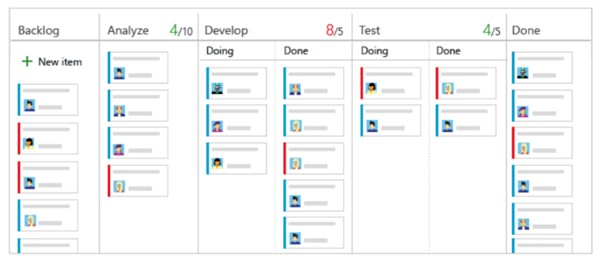
\includegraphics[scale=0.65]{Images/kanban_workflow.jpg}
    \caption{Kanban Workflow}
    \label{fig:kanban_workflow}
\end{figure}


\subsection{Development Process}
The project followed an iterative engineering cycle designed to balance thorough planning with incremental delivery, as illustrated in Figure~\ref{fig:development_cycle}. This cycle guided the work through structured stages, supported by dedicated tools and regular collaboration:

\begin{figure}[H]
    \centering
    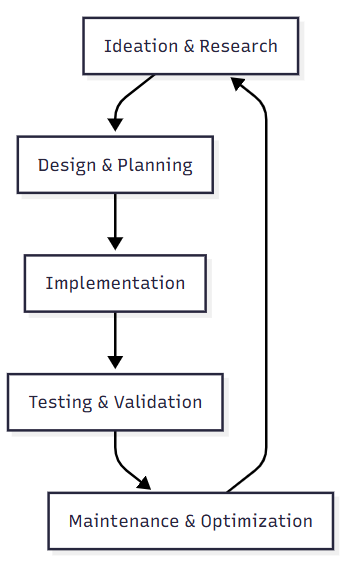
\includegraphics[scale=0.5]{Images/dev_process.png}
    \caption{Project Development Cycle}
    \label{fig:development_cycle}
\end{figure}

The main stages, as depicted in the figure, included:

\begin{itemize}
    \item \textbf{Onboarding and Initial Tasks:} The project began with a structured onboarding phase, where familiarization with internal tools, repositories, and coding standards was combined with the resolution of assigned bugs. This phase ensured a smooth transition into the team’s workflow and provided early practical experience.

    \item \textbf{Ideation and Research:} Following onboarding, the project entered an exploration phase to clarify objectives, gather requirements, and investigate potential solution directions. Independent research was complemented by collaborative discussions to assess feasibility and align priorities.

    \item \textbf{Design and Planning:} A detailed design document was authored to present technical choices, architectural considerations, and the proposed workflow. The document underwent iterative review by engineers, and the final approved plan was transferred to the internal task management system for structured tracking and prioritization.

    \item \textbf{Implementation:} Development was performed in small, reviewable increments using the internal development environment within the company-wide repository. Each change was submitted with unit tests and validated through manual and AI-assisted code reviews.

    \item \textbf{Testing and Validation:} Functionality and reliability were verified continuously. Automated unit tests ensured correctness at the component level, while integration reviews and structured evaluations validated the behavior within the larger system.

    \item \textbf{Maintenance and Optimization:} Refactoring, bug fixes, and updates were performed throughout development, particularly as dependencies evolved or methods became deprecated. This ensured that the solution remained consistent, maintainable, and aligned with evolving standards.
\end{itemize}

Collaboration was supported through a structured communication rhythm, combining regular syncs with the host and co-host, weekly team meetings, and occasional cross-team discussions. This cadence provided timely feedback, clear guidance, and alignment on shared dependencies throughout the iterative cycle.


\subsection{Project Timeline}
The project spanned four months (May 5 – September 5, 2025). Work was scheduled based on business priorities and technical dependencies. Early weeks focused on research and design, followed by implementation, testing, and iterative refinement.

% Landscape page for timeline
\newpage
\begin{landscape}
\vspace*{\fill}
\begin{figure}[!ht]
    \centering
    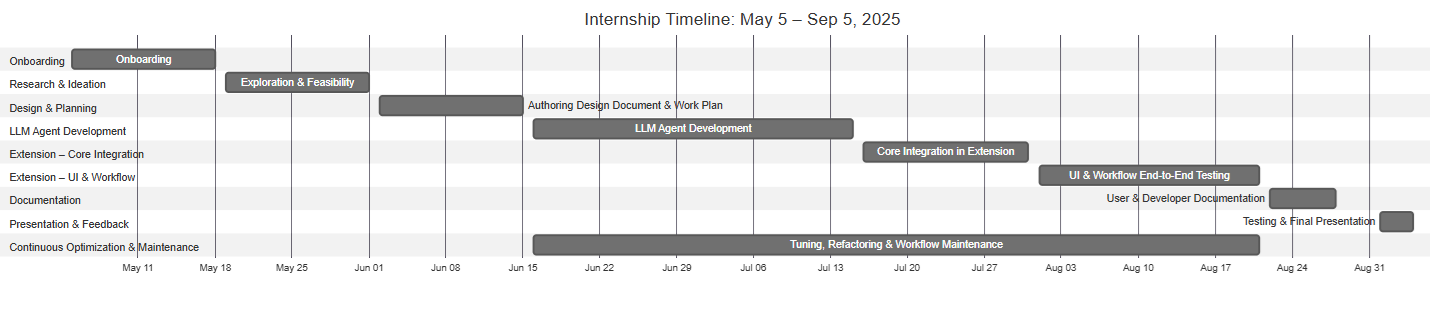
\includegraphics[width=1.3\textwidth,height=0.9\textheight,keepaspectratio]{Images/project_timeline.png}
    \caption{Project Timeline - Detailed Schedule}
    \label{fig:project_timeline}
\end{figure}
\vspace*{\fill}
\end{landscape}
\newpage


\section*{Conclusion}
In summary, this chapter outlined the project’s context by presenting the host company, defining the problem, and clarifying the main objectives and challenges. It also described the methodology chosen to guide the work, which provides the basis for the technical developments detailed in the following chapters.



%==============================================================================
\end{spacing}


\setcounter{chapter}{1}
\chapter{Business Understanding and State of the Art}
\minitoc %insert la minitoc
\graphicspath{{Chapitre2/figures/}}

%\DoPToC

%==============================================================================
\pagestyle{fancy}
\fancyhf{}
\fancyhead[R]{\bfseries\rightmark}
\fancyfoot[R]{\thepage}
\renewcommand{\headrulewidth}{0.5pt}
\renewcommand{\footrulewidth}{0pt}
\renewcommand{\chaptermark}[1]{\markboth{\MakeUppercase{\chaptername~\thechapter. #1 }}{}}
\renewcommand{\sectionmark}[1]{\markright{\thechapter.\thesection~ #1}}

\begin{spacing}{1.2}
%==============================================================================

\section*{Introduction}
This chapter establishes the theoretical and contextual foundation of the project. It begins with an overview of the Software Development Life Cycle (SDLC) and the emerging role of AI technologies such as Large Language Models (LLMs), Generative AI, and AI agents in modern software engineering. It then presents the state of the art, reviewing existing solutions that support code quality and best practices. Finally, it defines the project requirements, both functional and non-functional, showing how this work addresses gaps by integrating AI-driven assistance into key SDLC phases.

\section{Business and Reasoning}

\subsection{Software Development Life Cycle (SDLC)}
The Software Development Life Cycle (SDLC) provides a structured framework for planning, creating, testing, deploying, and maintaining software systems. As development teams grow and projects become more complex, maintaining code quality and consistency across all phases becomes increasingly challenging. As shown in Figure~\ref{fig:sdlc_cycle}, each phase presents unique challenges that can impact developer productivity and software reliability.

\begin{figure}[H]
    \centering
    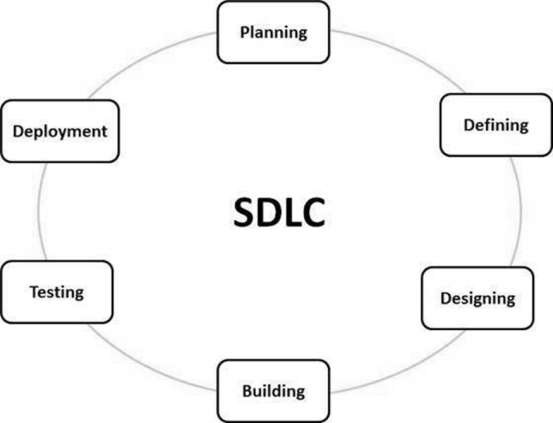
\includegraphics[scale=0.65]{Images/sdlc_stages.jpg}
    \caption{Software Development Life Cycle Overview}
    \label{fig:sdlc_cycle}
\end{figure}

\subsubsection*{Key Development Challenges}
Modern software development faces several critical challenges:

\begin{itemize}
    \item \textbf{Scalability Issues:} Maintaining consistent coding standards and best practices becomes increasingly difficult as teams grow, particularly without automated assistance.
    
    \item \textbf{Quality Assurance Gaps:} Traditional QA relies heavily on human review, introducing delays and inconsistent feedback timing.
    
    \item \textbf{Technical Debt Accumulation:} Without timely guidance, developers may adopt patterns that violate best practices, leading to accumulating technical debt.
    
    \item \textbf{Knowledge Transfer Challenges:} New team members often learn framework-specific conventions and best practices through trial and error, slowing onboarding and introducing variability.
\end{itemize}

\subsubsection*{Modern Development Approaches}
Contemporary practices aim to mitigate these challenges:

\begin{itemize}
    \item \textbf{Agile Methodologies:} Emphasize iterative development, continuous feedback, and rapid adaptation to changing requirements.
    
    \item \textbf{DevOps Integration:} Combines development and operations practices to enable continuous integration, automated testing, and real-time monitoring.
    
    \item \textbf{AI-Enhanced Development:} Emerging AI technologies provide intelligent assistance throughout the development process, from code generation to quality assurance.
\end{itemize}

These approaches lay the foundation for understanding how AI can address persistent challenges in code quality and consistency across modern software teams.

\subsection{Artificial Intelligence in Software Development}

\subsubsection*{Foundational AI Concepts}
Artificial Intelligence (AI) refers to computational systems capable of performing tasks that typically require human intelligence, such as reasoning, learning, problem-solving, and decision-making. AI encompasses a broad spectrum of techniques and paradigms with distinct capabilities and applications. Figure~\ref{fig:ai_hierarchy} provides a visual hierarchy of AI technologies.

\begin{figure}[H]
    \centering
    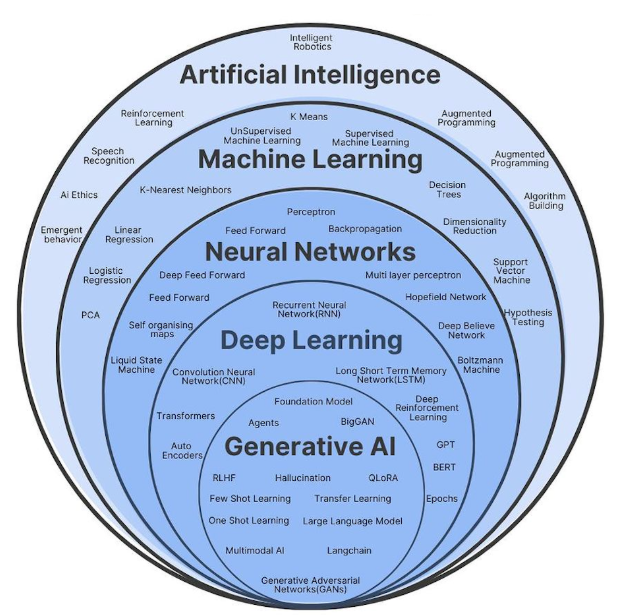
\includegraphics[scale=0.6]{Images/AI.png}
    \caption{Hierarchy of AI Technologies}
    \label{fig:ai_hierarchy}
\end{figure}

Key categories include:

\begin{itemize}
    \item \textbf{Symbolic AI:} Rule-based systems for reasoning and knowledge representation.
    \item \textbf{Machine Learning (ML):} Algorithms that learn from data to improve task performance.
    \item \textbf{Deep Learning (DL):} Neural networks with multiple layers capable of modeling complex patterns.
    \item \textbf{Generative AI:} Systems that produce new content, such as text or code, by learning patterns from existing datasets.
\end{itemize}

\subsubsection*{The AI Revolution in Software Engineering}
As software development becomes increasingly complex, traditional approaches struggle to maintain quality while meeting delivery deadlines. AI technologies offer transformative opportunities by embedding intelligent assistance directly into the development workflow.

Industry adoption illustrates this impact: surveys indicate that AI-generated code accounts for a significant portion of development output in major tech organizations~\cite{google2024ai_code, google2024developer_survey}. AI integration addresses critical business challenges, including maintaining code quality, reducing technical debt, and scaling development practices across growing teams. This shift defines the AI-Enhanced SDLC, a lifecycle where intelligent assistance is embedded throughout all phases.

\subsubsection*{Large Language Models (LLMs)}
LLMs represent a breakthrough in generative AI, trained on extensive natural language and code corpora. Unlike traditional tools, they understand context, semantics, and intent, enabling complex reasoning across domains. Figure~\ref{fig:llm_overview} shows a chronological overview of LLM development from 2018–2024.

\begin{figure}[H]
    \centering
    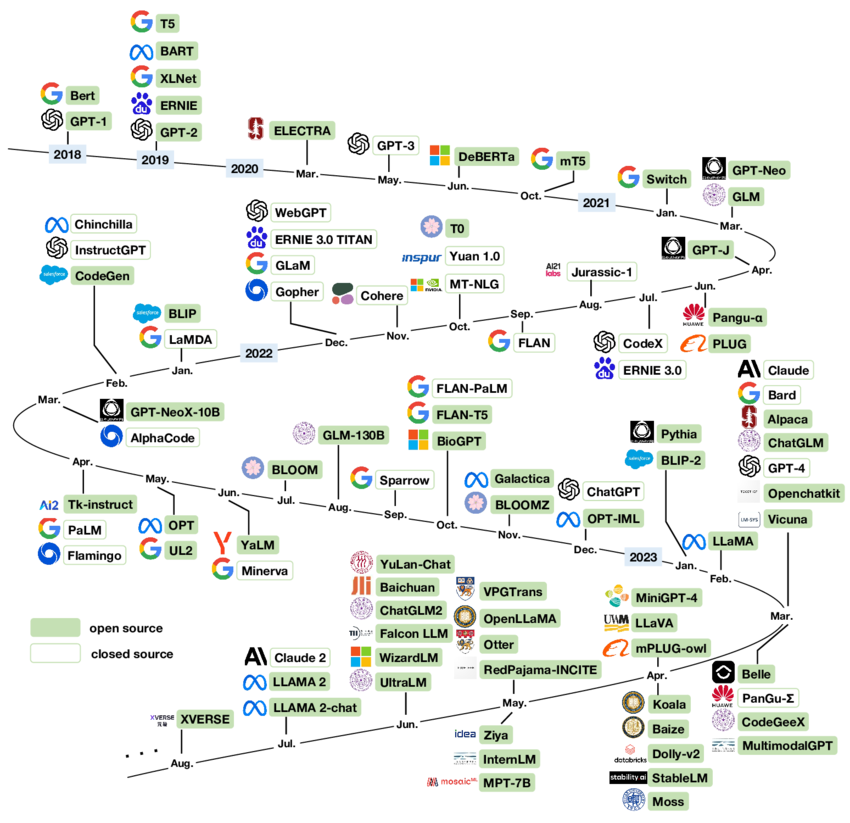
\includegraphics[scale=1]{Images/A-chronological-overview-of-large-language-models-LLMs-multimodal-and-scientific.png}
    \caption{Chronological Overview of Large Language Models (LLMs)}
    \label{fig:llm_overview}
\end{figure}

LLM capabilities include:

\begin{itemize}
    \item \textbf{Natural Language Understanding}
    \item \textbf{Pattern Recognition}
    \item \textbf{Content Generation}
    \item \textbf{Reasoning and Inference}
\end{itemize}

Applied to software development, these translate into:

\begin{itemize}
    \item \textbf{Contextual Code Analysis}
    \item \textbf{Intelligent Code Generation}
    \item \textbf{Explanatory Documentation}
    \item \textbf{Semantic Standards Enforcement}
\end{itemize}

\subsubsection*{AI Agents}
AI agents build on LLMs by autonomously reasoning, planning, and executing development tasks. They orchestrate LLM capabilities within workflows, providing seamless integration into IDEs, testing frameworks, and version control systems. Figure~\ref{fig:ai_agent_workflow} illustrates the agent architecture and orchestration workflow.

\begin{figure}[H]
    \centering
    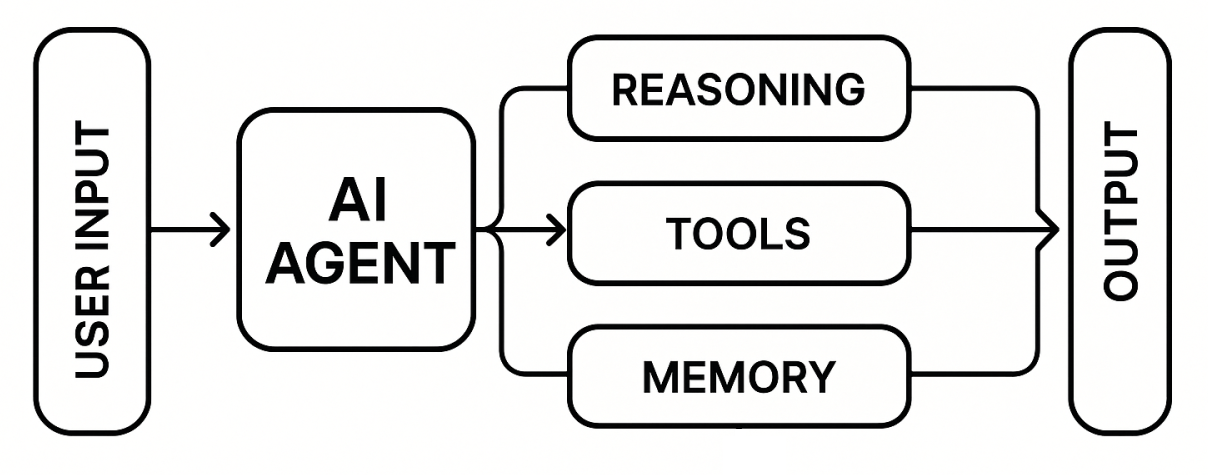
\includegraphics[scale=0.2]{Images/ai_agent.png}
    \caption{AI Agent Architecture and Orchestration Workflow}
    \label{fig:ai_agent_workflow}
\end{figure}

Core components include:

\begin{itemize}
    \item Code Analysis Engine
    \item Contextual Reasoning
    \item Development Tool Integration
    \item Contextual Adaptation via system prompts
    \item Feedback and Explanation System
\end{itemize}

\subsubsection*{Balancing AI Capabilities and Practical Considerations}
\textbf{Capabilities:}
\begin{itemize}
    \item Contextual Understanding
    \item Automated Analysis
    \item Intelligent Recommendations
    \item Project-specific Adaptation
\end{itemize}

\textbf{Limitations:}
\begin{itemize}
    \item Computational Cost
    \item Context Constraints
    \item Accuracy Considerations
    \item Integration Complexity
    \item Adaptation via prompts rather than continuous learning
\end{itemize}

\subsubsection*{AI-Enhanced SDLC}
The combination of LLMs and AI agents enables proactive, intelligent assistance throughout the entire software development lifecycle. This AI-enhanced SDLC transforms traditional development practices by embedding guidance, analysis, and automated support at each phase.

\paragraph{Transformative Impact on Development Practices}
\begin{itemize}
    \item \textbf{From Reactive to Proactive:} Traditional workflows provide feedback mainly during code reviews or testing phases. AI-enhanced systems deliver guidance during coding, design, and planning, preventing issues before they become embedded in the codebase and reducing the need for extensive refactoring.
    
    \item \textbf{From Inconsistent to Scalable:} Human-based quality assurance can vary in expertise and availability. AI agents provide consistent, expert-level analysis across large teams and codebases, ensuring uniform adherence to best practices and internal framework conventions.
    
    \item \textbf{From Static to Adaptive:} Unlike rule-based tools, AI adapts to project-specific patterns, team preferences, and evolving best practices, offering context-aware suggestions tailored to the particular codebase.
    
    \item \textbf{From Isolated to Integrated:} Instead of treating quality assurance and guidance as separate phases, AI agents integrate intelligent support directly into developer workflows, bridging planning, implementation, testing, and maintenance.
\end{itemize}

\paragraph{AI Applications Across the SDLC}
AI technologies provide targeted assistance at each SDLC phase, addressing specific challenges and improving efficiency:

\begin{itemize}
    \item \textbf{Requirements and Planning:} AI analyzes historical project data to estimate timelines, identify ambiguities in requirements, and suggest optimal resource allocation. Natural language processing helps translate business requirements into technical specifications with higher precision.
    
    \item \textbf{Design and Architecture:} AI assists architects by analyzing existing codebases, recommending architectural patterns, detecting design anti-patterns, and ensuring alignment with organizational standards. This reduces the likelihood of systemic flaws early in the project lifecycle.
    
    \item \textbf{Implementation:} During coding, AI agents provide context-aware code completions, enforce framework-specific best practices, detect potential bugs, and suggest refactoring opportunities. This reduces rework, accelerates development, and supports consistent code quality.
    
    \item \textbf{Testing and Quality Assurance:} AI generates comprehensive test cases, identifies edge cases that might be missed manually, prioritizes test execution based on risk, and evaluates code quality against defined standards. This enhances reliability and reduces technical debt accumulation.
    
    \item \textbf{Deployment and Maintenance:} AI monitors deployment health, predicts potential issues, and recommends optimizations based on performance metrics and usage patterns. Continuous insights help maintain system stability and inform future development iterations.
\end{itemize}

Overall, the AI-enhanced SDLC shifts the development workflow from reactive and fragmented practices toward a more proactive, adaptive, and integrated approach. By embedding intelligent assistance at every stage, it directly addresses the challenges of scaling teams, maintaining consistent quality, and supporting internal framework-specific best practices—core objectives of this project.

\section{State of the Art and Existing Solutions}

This section examines both market-available solutions (state of the art) and environment-specific approaches (existing solutions) to understand the current landscape of code quality and best practices enforcement.

\subsection{State of the Art: Market Solutions}

The software development market offers various AI-powered tools and platforms that aim to enhance code quality and developer productivity. These solutions represent the current state of the art in intelligent development assistance:

\paragraph{AI-Powered Code Analysis Tools}
Commercial and open-source solutions provide intelligent code analysis capabilities:

\begin{itemize}
    \item \textbf{AI Code Assistants:} Tools like GitHub Copilot, Amazon CodeWhisperer, and Tabnine provide AI-powered code completion and generation, helping developers write code more efficiently.
    
    \item \textbf{AI-Powered IDEs:} Modern development environments like Cursor and Claude Code integrate AI assistance directly into the coding workflow, offering context-aware code generation, refactoring, and intelligent suggestions.
    
    \item \textbf{Static Analysis Platforms:} Solutions such as SonarQube, CodeClimate, and DeepCode offer automated code quality analysis with AI-enhanced pattern detection.
    
    \item \textbf{AI Code Review Tools:} Platforms like PullRequest.com and CodeRabbit provide AI-assisted code review capabilities, offering automated suggestions and quality assessments.
\end{itemize}

\paragraph{Market Solution Capabilities}
These market solutions typically offer:

\begin{itemize}
    \item \textbf{General Code Analysis:} Broad pattern recognition and quality assessment across multiple programming languages and frameworks.
    
    \item \textbf{AI-Powered Suggestions:} Intelligent recommendations for code improvements, refactoring, and best practices.
    
    \item \textbf{Integration with Popular IDEs:} Seamless integration with widely-used development environments like VS Code, IntelliJ, and Eclipse.
\end{itemize}

\subsection{Existing Solutions: Environment-Specific Approaches}

Within our specific development environment, software engineers currently rely on a combination of modern AI-powered tools and traditional approaches to maintain code quality and enforce best practices:

\paragraph{Current Feedback Mechanisms}
The existing approaches in our environment can be categorized into several key mechanisms:

\begin{itemize}    
    
    \item \textbf{Code Reviews:} Human reviewers examine code for design quality, readability, maintainability, and adherence to standards. While this approach provides high-level, context-aware feedback, it often introduces delays and requires significant effort.
    
    \item \textbf{Presubmit Checks:} Automated scripts that validate code before submission, enforcing style guides, ensuring compilation, and verifying simple correctness and safety constraints. Although fast and reliable, they primarily focus on surface-level checks and do not consider design or contextual issues.
    
    \item \textbf{Coding Assistant:} Our internal IDE includes an integrated coding assistant that provides AI-powered code completion, generation, and basic suggestions to help developers write code more efficiently.

    \item \textbf{Linters:} Live IDE-integrated linters that catch style issues, deprecations, and basic code quality problems in real-time as developers write code. These tools provide immediate feedback on syntax, formatting, and some best practices.

    \item \textbf{Rule-Based Checks:} Systems that enforce coding conventions, naming schemes, and formatting standards. These tools provide consistency and objectivity but cannot reason about complex or context-dependent best practices.
\end{itemize}

\paragraph{Gap Analysis: Market vs. Environment Solutions}

While both market solutions and environment-specific approaches provide valuable capabilities, they leave significant gaps in addressing internal framework-specific best practices:

\textbf{Market Solution Limitations:}
\begin{itemize}
    \item \textbf{Generic Analysis:} Market tools provide general code quality analysis but lack deep understanding of internal framework-specific conventions and patterns.
    
    \item \textbf{External Dependency:} Commercial solutions require external data sharing and may not align with internal security and privacy requirements.
    
    \item \textbf{Limited Customization:} Generic tools cannot be easily customized to enforce internal-specific best practices and architectural patterns.
\end{itemize}

\textbf{Environment Solution Limitations:}
While our environment includes a coding assistant and live linters, there remains a significant gap in providing intelligent feedback specifically for internal framework best practices during the active coding phase. This timeline illustrates where current feedback mechanisms fit into the developer workflow:

\begin{figure}[H]
    \centering
    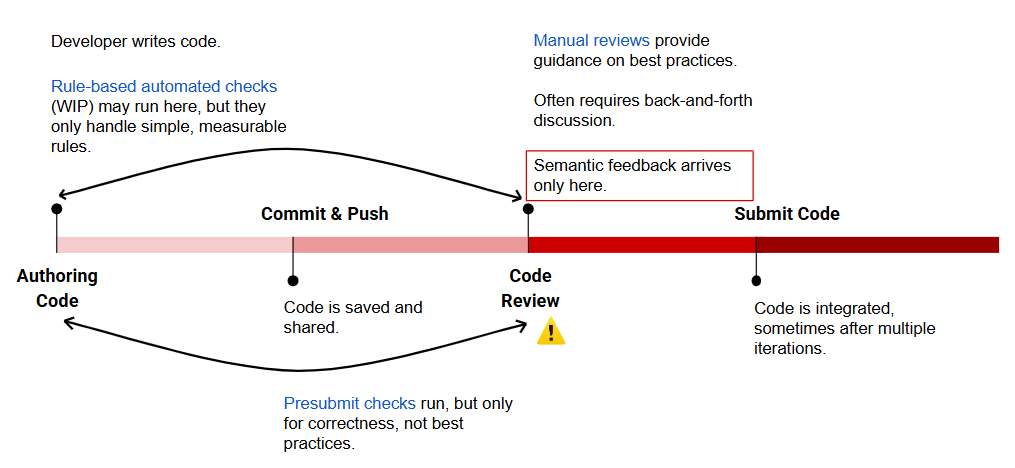
\includegraphics[scale=0.9]{Images/developer_workflow_feedback_timeline.png}
    \caption{Current Developer Workflow Feedback Timeline}
    \label{fig:developer_workflow_feedback_timeline}
\end{figure}

During the \textbf{Coding Phase}, developers get support from the Coding Assistant for code generation and completion, and from Linters for style issues and deprecations. However, these tools focus on general coding assistance and basic quality checks rather than internal framework-specific best practices.

The most insightful feedback on design and best practices typically comes during \textbf{Code Review}, but this happens after the initial development, making changes more disruptive.

Finally, \textbf{Presubmit Checks} before submission focus on correctness and safety, not on proactive best practice guidance.

This leaves a significant gap: there's no real-time, intelligent support for adhering to internal framework best practices while the developer is actively coding, which is the gap our project aims to fill.

\begin{table}[H]
\centering
\begin{tabular}{|p{4cm}|p{5cm}|p{5cm}|}
\hline
\textbf{Approach} & \textbf{Strengths} & \textbf{Limitations} \\
\hline
Code Reviews & Context-aware, high-level insights & Feedback delayed, time-consuming \\
\hline
Presubmit Checks & Fast, automated validation & Limited scope, mostly syntax and safety \\
\hline
Coding Assistant & AI-powered code generation, completion & General assistance, not framework-specific \\
\hline
Linters & Real-time style and deprecation checks & Basic quality only, not best practices \\
\hline
Rule-Based Checks & Consistency, objectivity & Cannot handle complex or contextual practices \\
\hline
\end{tabular}
    \caption{Comparison of available software quality support solutions}
\label{tab:extended_solutions}
\end{table}

    
\paragraph{Impact of Delayed Feedback}
Following from the previous analysis, these workflow issues create concrete impacts on development:

\begin{itemize}
    \item \textbf{Technical Debt Accumulation:} Delayed feedback and limited enforcement of best practices lead to accumulating technical debt and inconsistencies in code quality over time.
    
    \item \textbf{Prolonged Review Cycles:} Review cycles take longer because developers must iterate multiple times to address issues discovered late in the process.
    
    \item \textbf{Developer Frustration:} The repetitive cycle of late-stage corrections contributes to developer frustration and reduced productivity.
    
    \item \textbf{Inconsistent Quality Standards:} Without real-time guidance, adherence to best practices varies significantly across team members and projects.
    
    \item \textbf{Increased Development Costs:} The cost of fixing issues increases exponentially the later they are discovered in the development process.
\end{itemize}

This analysis clearly demonstrates why we need a solution that brings intelligent best practices guidance earlier, directly into the authoring process, addressing the specific gap in internal framework best practices enforcement that current approaches cannot fill.




\paragraph{Opportunity for Framework-Specific AI Solutions}

The analysis reveals a clear opportunity for developing framework-specific AI solutions that combine the intelligence of market tools with the specificity required for YouTube framework best practices. While market solutions provide general AI capabilities and environment solutions offer domain knowledge, neither adequately addresses the need for real-time, intelligent feedback tailored to YouTube framework conventions.

This gap creates a compelling case for integrating LLM-powered assistance directly into the YouTube development workflow, providing intelligent, context-aware guidance that understands both general best practices and YouTube-specific patterns.

---

\section{Project Requirements}

To tackle the issue of delayed feedback and limited intelligent assistance, our solution integrates the power of large language models directly into the developer's workflow in the IDE.

The proposed system builds on gaps identified in existing solutions. It aims to provide real-time, AI-driven feedback directly in the developer workflow, while maintaining performance, scalability, and usability.

\subsection{Functional Requirements}
The system must:
\begin{itemize}
    \item \textbf{Detect Framework Violations:} Identify violations of internal YouTube framework best practices and coding standards in real-time during development.
    
    \item \textbf{Provide Contextual Explanations:} Explain violations in clear, developer-friendly language with context-specific rationale that helps developers understand why certain patterns are problematic.
    
    \item \textbf{Generate Actionable Fixes:} Suggest specific, actionable fixes leveraging AI-generated solutions tailored to YouTube framework patterns and conventions.
    
    \item \textbf{Enable Developer Interaction:} Allow developers to accept, reject, or modify AI suggestions, providing full control over the implementation of recommended changes.
    
    \item \textbf{Maintain Contextual Relevance:} Ensure feedback appears in the appropriate location within the code and remains relevant and accurate as the developer continues coding.
    
    \item \textbf{Seamless IDE Integration:} Integrate seamlessly with the existing internal IDE, extension, and backend workflow without disrupting the developer's current development process.
\end{itemize}

\subsection{Non-Functional Requirements}
The system should also meet broader quality criteria:
\begin{itemize}
    \item \textbf{Performance:} Provide fast, near real-time responses to avoid interrupting developer workflow.
    \item \textbf{Scalability:} Efficiently handle large codebases and multiple simultaneous users.
    \item \textbf{Maintainability:} Enable modular updates, addition of new AI models, or coding rules.
    \item \textbf{Reliability:} Ensure robustness in production environments with minimal downtime.
    \item \textbf{Security and Privacy:} Comply with organizational policies, ensuring safe handling of code and data.
    \item \textbf{Usability:} Deliver concise, context-aware, and minimally intrusive feedback.
    \item \textbf{Extensibility:} Easily add new rules, models, or integrations.
\end{itemize}

\begin{table}[H]
\centering
\begin{tabular}{|p{6cm}|p{8cm}|}
\hline
\textbf{Requirement Type} & \textbf{Description} \\
\hline
Functional & Framework violation detection, contextual explanations, actionable fixes, developer interaction, contextual relevance, seamless IDE integration \\
\hline
Non-Functional & Performance, scalability, maintainability, reliability, security, usability, extensibility \\
\hline
\end{tabular}
\caption{Summary of project requirements}
\label{tab:extended_requirements}
\end{table}

\paragraph{Rationale}
These requirements address limitations identified in existing solutions by embedding proactive, context-aware feedback directly in the coding workflow, specifically targeting YouTube framework best practices. This approach enhances developer productivity, reduces framework-specific errors, and supports consistent adherence to internal YouTube development standards.


\section*{Conclusion}
This chapter established the business and theoretical foundation for integrating AI into YouTube framework development workflows. Beginning with an analysis of modern development challenges, it identified key issues in maintaining code quality and consistency across growing teams. The exploration of AI technologies—particularly Large Language Models and AI agents—revealed their potential for addressing these challenges through proactive, context-aware assistance.

The examination of both market solutions and environment-specific approaches highlighted significant limitations: market tools lack framework-specific knowledge, while traditional environment solutions provide delayed feedback and limited scope. There remains a critical gap in delivering real-time, intelligent assistance tailored to YouTube framework best practices.

The project requirements defined in this chapter focus on bridging this gap through real-time, AI-driven feedback that integrates seamlessly into the YouTube development workflow. The proposed solution combines the intelligence of modern AI technologies with the specificity required for YouTube framework conventions, setting the stage for the detailed system design presented in the following chapter.  








%==============================================================================
\end{spacing}




\setcounter{chapter}{2}
\chapter{System Design and Architecture}
\minitoc %insert la minitoc
\graphicspath{{Chapitre3/figures/}}

%\DoPToC
%==============================================================================
\pagestyle{fancy}
\fancyhf{}
\fancyhead[R]{\bfseries\rightmark}
\fancyfoot[R]{\thepage}
\renewcommand{\headrulewidth}{0.5pt}
\renewcommand{\footrulewidth}{0pt}
\renewcommand{\chaptermark}[1]{\markboth{{\chaptername~\thechapter. #1 }}{}}
\renewcommand{\sectionmark}[1]{\markright{\thechapter.\thesection~ #1}}

\begin{spacing}{1.2}

%==============================================================================
\section*{Introduction}
This chapter presents the system design and architecture of the LLM-powered best practices enforcement system. Building on the business understanding and requirements established in the previous chapter, this chapter details the technical design decisions, architectural patterns, and system components that enable real-time, intelligent feedback for YouTube framework development.

The design follows traditional software engineering principles while incorporating modern AI technologies. This chapter covers the overall system architecture, component design, data models, and integration patterns that form the foundation of the implemented solution.

\section{System Architecture Overview}


\subsection{Use Case Analysis}

Understanding the system's interactions with its users is fundamental to designing an effective solution. The use case analysis identifies the primary actors and their interactions with the LLM Best Practices Enforcement System, establishing the scope and boundaries of the system's functionality.

\begin{figure}[H]
\centering
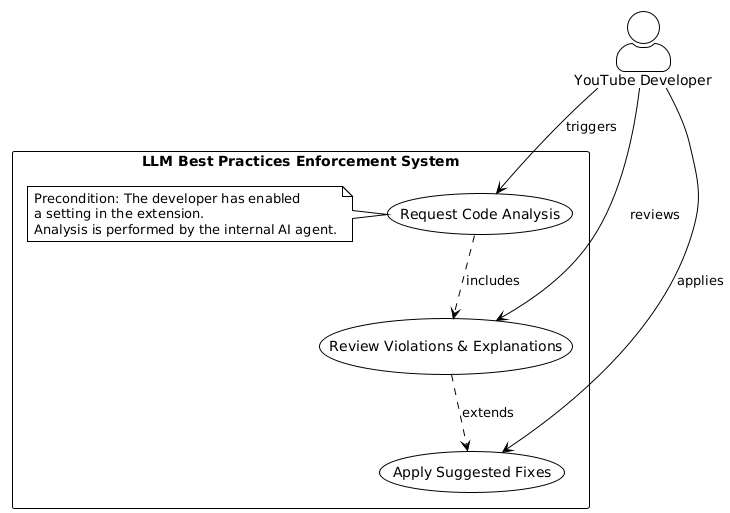
\includegraphics[scale=0.6]{images/use_case_diagram.png}
\caption{System Use Case Diagram}
\label{fig:use_case_diagram}
\end{figure}

This use case diagram illustrates the core functionality of the system from the perspective of YouTube developers. The primary actor is the YouTube Developer, who interacts with the system through three main use cases: requesting code analysis, reviewing violations and explanations, and optionally applying suggested fixes. The relationship between use cases reflects the natural workflow: analysis always includes reviewing results, while applying fixes is an optional extension that developers can choose based on their needs and preferences. This design ensures that developers maintain control over their workflow while providing comprehensive feedback when requested. The diagram focuses on the most important scenarios that occur during normal system usage, avoiding authentication and administrative scenarios that are less central to the user experience.


\subsection{High-Level Architecture}
The system architecture is designed to integrate seamlessly into the developer's existing workflow while providing intelligent, context-aware feedback. The architecture consists of two main components that work together to deliver real-time best practice enforcement:

\begin{itemize}
    \item \textbf{IDE}: The developer's workspace containing the YouTube IDE Extension, which works with the currently open file being analyzed and annotates results directly in the editor.
    \item \textbf{AI Agent Framework}: The processing layer containing the LLM Best Practices Agent, which serves as the core AI processing engine that uses internal LLMs to analyze code and suggest best practices.
\end{itemize}

\begin{figure}[H]
\centering
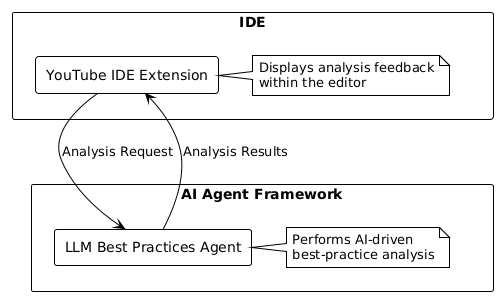
\includegraphics[scale=0.7]{images/high_level_system_architecture.png}
\caption{High-Level System Architecture}
\label{fig:system_architecture}
\end{figure}

This architecture diagram illustrates the fundamental separation between the user-facing IDE extension and the AI processing backend. The YouTube IDE Extension operates within the developer's workspace, providing immediate access to analysis capabilities while maintaining the familiar development environment. The AI Agent Framework handles the computationally intensive analysis tasks, ensuring that the IDE remains responsive during processing. This separation enables independent scaling of AI capabilities without impacting the development environment's performance.

\subsection{System Workflow}
The system operates through a streamlined workflow that begins when a developer triggers analysis via the YouTube IDE Extension. The complete interaction flow is depicted in Figure \ref{fig:sequence_diagram}.

\begin{figure}[H]
\centering
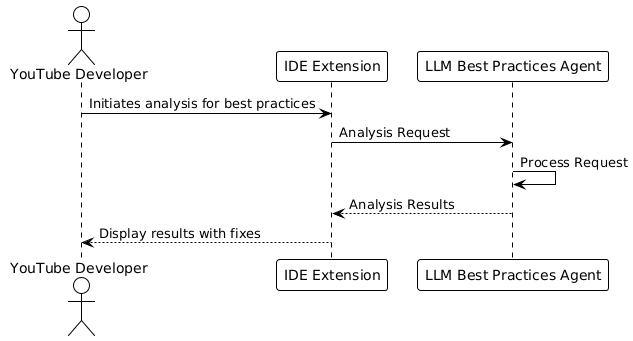
\includegraphics[scale=0.7]{images/sequence_diagram.png}
\caption{System Interaction Sequence Diagram}
\label{fig:sequence_diagram}
\end{figure}

This sequence diagram captures the most important interaction scenario: a developer requesting analysis of their current file. The diagram shows the complete flow from user action to result presentation, demonstrating how the system maintains responsiveness by delegating heavy processing to the AI agent while providing immediate feedback through the IDE extension. This represents the primary use case that occurs most frequently in the system.

The sequence unfolds through the following interactions and responsibilities:
\begin{enumerate}
    \item \textbf{Analysis initiation}: The YouTube developer triggers analysis of the currently open file.
    \item \textbf{Request submission}: The YouTube IDE Extension submits an analysis request to the agent, identifying the target file.
    \item \textbf{Processing}: The agent performs best-practices analysis and prepares the resulting findings.
    \item \textbf{Result delivery}: The agent returns a structured response to the YouTube IDE Extension.
    \item \textbf{Presentation}: The YouTube IDE Extension presents the best practices violations and suggested fixes within the editor.
\end{enumerate}

This workflow emphasizes decoupling the IDE from heavy AI computation, ensuring that the development environment remains responsive while delegating intensive analysis to the specialized agent framework.

\section{Components Design}

\subsection{LLM Best Practices Agent} 
The LLM Best Practices Agent serves as the core intelligence engine of the system, responsible for analyzing code, identifying violations of YouTube framework best practices, and providing actionable feedback to developers. This component represents the convergence of modern AI capabilities with domain-specific software engineering expertise.

\subsubsection{Agent Architecture Choice}
The agent is built using the \textit{Executable Agent} architecture~\cite{microsoftAgentPatterns}, provided by our internal AI platform. This architecture offers a structured approach to orchestrating AI-powered workflows, and was selected after careful evaluation of different agent paradigms, considering reliability, performance, and maintainability.

\paragraph{Executable Agent vs. ReAct Architecture}
To motivate the choice of \textit{Executable Agent} architecture, we contrast it with the more widely known ReAct (Reasoning and Acting) pattern. In our system, the \textit{Executable Agent} refers to a deterministic, tool-orchestrated workflow where control flow is defined in code rather than delegated to LLM reasoning.

\begin{itemize}
    \item \textbf{ReAct Agent}: Uses a reasoning loop where the LLM decides what action to take next, executes it, observes the result, and continues reasoning. This creates a dynamic, LLM-driven execution flow.
    \item \textbf{Executable Agent}: Follows a predefined, deterministic execution flow where the agent orchestrates a sequence of tool calls in a structured manner, with the LLM used primarily for processing within each tool rather than for orchestration decisions.
\end{itemize}


Figure~\ref{fig:agent_comparison} illustrates the fundamental difference in control flow between the two approaches.

\begin{figure}[H] 
	\centering 
	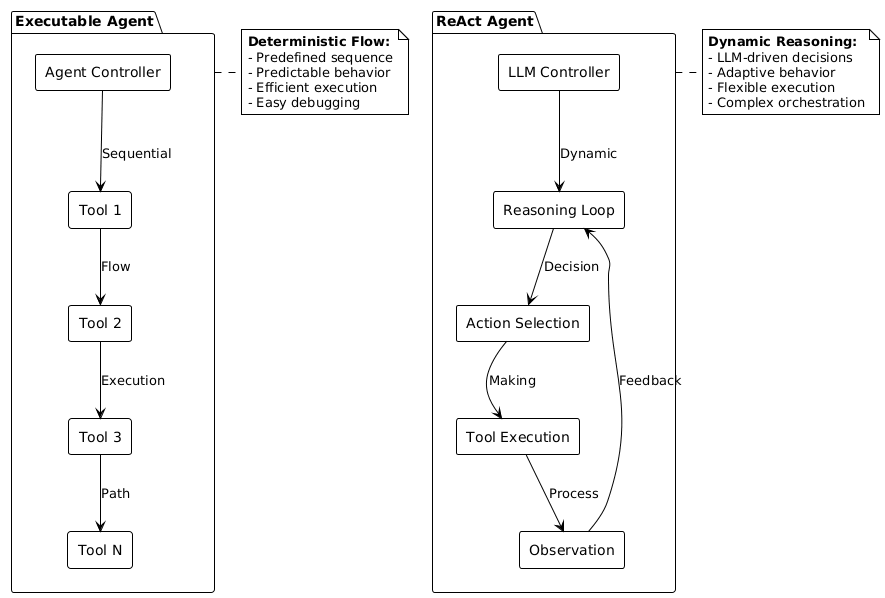
\includegraphics[scale=0.6]{images/agent_architecture_comparison.png} 
	\caption{Comparison of Executable Agent vs. ReAct Agent Architectures} 
	\label{fig:agent_comparison} 
\end{figure}

The Executable Agent architecture offers several key advantages for this use case:
\begin{itemize}
    \item \textbf{Deterministic Execution}: Predefined flow ensures predictable behavior and simplifies debugging.
    \item \textbf{Tool Orchestration}: Clean framework for coordinating multiple specialized tools.
    \item \textbf{Error Handling}: Built-in mechanisms for handling failures and graceful degradation.
    \item \textbf{Performance}: Efficient execution with low response latency, since orchestration decisions are pre-programmed rather than deferred to open-ended LLM reasoning.
    \item \textbf{Cost Efficiency}: Reduced token consumption by constraining LLM calls to focused, well-scoped processing steps rather than repeated reasoning loops.
    \item \textbf{Maintainability}: Clear separation of concerns between tools and responsibilities.
\end{itemize}



\subsubsection{Core Tools Architecture}
To achieve this structured workflow, the agent incorporates five specialized tools, each handling a specific step of the best practices analysis pipeline.

\paragraph{Tool Responsibilities}
The agent's tool architecture follows a sequential workflow where each tool has a distinct responsibility:

\begin{itemize}
    \item \textbf{File Reading Tool}: Responsible for retrieving the complete content of the file being analyzed, ensuring the agent has access to the full context of the code under examination.
    
    \item \textbf{Code Analysis Tool}: The core analysis engine that performs violation detection against YouTube framework best practices using semantic code analysis to understand intent and context.
    
    \item \textbf{Violation Explanation Tool}: Generates human-readable explanations for each identified violation, providing developers with clear understanding of why particular code patterns violate best practices.
    
    \item \textbf{Code Fix Tool}: Proposes actionable fix suggestions for identified violations, going beyond problem identification to provide concrete solutions that developers can implement.
    
    \item \textbf{Result Consolidation Tool}: Aggregates all analysis results into a structured output format, ensuring the response contains all necessary information for the IDE extension to display results effectively.
\end{itemize}

This tool-based architecture provides clear separation of concerns, with each tool handling a specific aspect of the analysis pipeline while maintaining a cohesive workflow. 
\subsubsection{Processing Strategy}
The agent employs a balanced processing strategy that weighs performance against reliability. This strategy represents a key architectural decision made after evaluating different processing approaches for handling multiple violations within a single file.

\paragraph{Processing Strategy Options}
During the design phase, three main processing strategies were considered for handling multiple violations:

\begin{itemize}
    \item \textbf{Fully Sequential Processing}: Each violation is processed one at a time, ensuring maximum reliability and predictability but potentially resulting in longer processing times for files with many violations.
    
    \item \textbf{Fully Parallel Processing}: All violations are processed concurrently, maximizing performance but introducing complexity in managing concurrent operations and potential reliability challenges under high load conditions.
    
    \item \textbf{Hybrid Processing Strategy}: A balanced approach that processes violations efficiently while maintaining system stability. This strategy provides significant performance improvements over sequential processing while ensuring reliable operation under various load conditions.
\end{itemize}

The hybrid processing strategy was selected as it provides the optimal balance between performance and reliability for production use. This strategy ensures that the agent can handle complex analysis tasks efficiently while maintaining system stability and providing consistent results.

\subsubsection{Integration with LLM Infrastructure}
The agent integrates with an internal AI platform that hosts multiple LLM models. The architecture is model‑agnostic, enabling seamless adoption of newer models as they are released without requiring changes in the orchestration logic. LLM usage is isolated behind stable interfaces so higher‑level logic remains unaffected. The analysis tools depend on the LLM for semantic understanding and code generation. This design ensures long‑term maintainability and benefits from platform improvements without architectural change.

\subsection{YouTube IDE Extension}
The YouTube IDE Extension serves as the user-facing interface that seamlessly integrates the LLM Best Practices Agent into YouTube developers' daily workflow. Since YouTube developers are the primary target audience for this system, the YouTube IDE Extension was chosen as the natural entry point, leveraging their existing development environment and workflow patterns. This component is designed to provide intelligent, context-aware feedback while maintaining the responsiveness and familiarity that developers expect from their development environment. The feature becomes available when developers enable a user setting in the extension, and entry points only appear for files that belong to the internal YouTube framework for which we enforce best practices.

\subsubsection{Extension Architecture}
The YouTube IDE Extension serves as a lightweight client that orchestrates the interaction between developers and the AI analysis system. The architecture ensures responsiveness by delegating computationally intensive analysis to the specialized agent framework while handling user interface concerns, progress indication, and result presentation locally.

\subsubsection{User-Triggered vs. Automatic Analysis Design Decision}
A fundamental design decision for the IDE extension was whether to implement user-triggered analysis or automatic analysis. This choice significantly impacts user experience, system performance, and resource utilization.

The primary motivation for user-triggered analysis stems from the need to maintain developer productivity and system efficiency. LLM analysis is computationally expensive and resource-intensive, making continuous analysis impractical for maintaining IDE responsiveness. User-triggered analysis ensures that analysis occurs only when developers specifically request it, providing contextually relevant feedback at optimal moments without interrupting their workflow. This approach aligns with developer expectations of having control over their development environment while ensuring that computational resources are used efficiently.

Table \ref{tab:analysis_approaches} summarizes the trade-offs:

\begin{table}[H]
\centering
\caption{Comparison of User-Triggered vs. Automatic Analysis Approaches}
\label{tab:analysis_approaches}
\begin{tabular}{|l|c|c|}
\hline
\textbf{Criteria} & \textbf{User-Triggered} & \textbf{Automatic} \\
\hline
User Control & $\checkmark$ & $\times$ \\
\hline
Resource Efficiency & $\checkmark$ & $\times$ \\
\hline
IDE Performance & $\checkmark$ & $\times$ \\
\hline
Contextual Timing & $\checkmark$ & $\times$ \\
\hline
Discoverability & $\times$ & $\checkmark$ \\
\hline
Always Current & $\times$ & $\checkmark$ \\
\hline
\end{tabular}
\end{table}

Based on this analysis, the user-triggered approach was selected as it provides superior resource management, user control, and system performance. The trade-offs in discoverability and stale state management are addressed through intuitive UI design and comprehensive feedback mechanisms.

\paragraph{Stale State Challenge}
The user-triggered approach introduces a fundamental design challenge: maintaining the relevance and accuracy of analysis results as developers continue modifying their code. This challenge requires balancing system responsiveness with result accuracy, ensuring that feedback remains useful throughout the development process.

\subsubsection{User Interface Design}
The YouTube IDE Extension is designed around two core interaction patterns: entry points for initiating analysis and feedback mechanisms for presenting results.

\paragraph{Entry Points}
The YouTube IDE Extension provides multiple entry points to ensure accessibility and discoverability for different user preferences and workflows:

\begin{itemize}
    \item \textbf{Visual Interface Integration}: Visual indicators are integrated into the development environment to provide immediate visibility of AI analysis availability, ensuring maximum discoverability while maintaining a clean interface.
    
    \item \textbf{Command-Based Access}: For developers who prefer keyboard-driven workflows, the extension provides command-based access through standard IDE navigation patterns, supporting both mouse-driven and keyboard-driven user interactions.
\end{itemize}

\paragraph{Feedback Mechanisms}
The YouTube IDE Extension employs three core feedback mechanisms designed to integrate seamlessly with existing development workflows:

\begin{itemize}
    \item \textbf{Progress Indication}: Real-time status updates during analysis processing to maintain developer awareness and system transparency.
    
    \item \textbf{Violation Display}: Presentation of analysis results using familiar interface patterns that leverage developers' existing knowledge of standard feedback mechanisms.
    
    \item \textbf{Contextual Suggestions}: Interactive code solutions that appear when developers interact with violation markers, providing actionable recommendations.
\end{itemize}


\subsubsection{User Interaction Flow}
The user interaction flow with the YouTube IDE Extension follows a structured pattern from analysis initiation to optional fix application:

\begin{figure}[H]
\centering
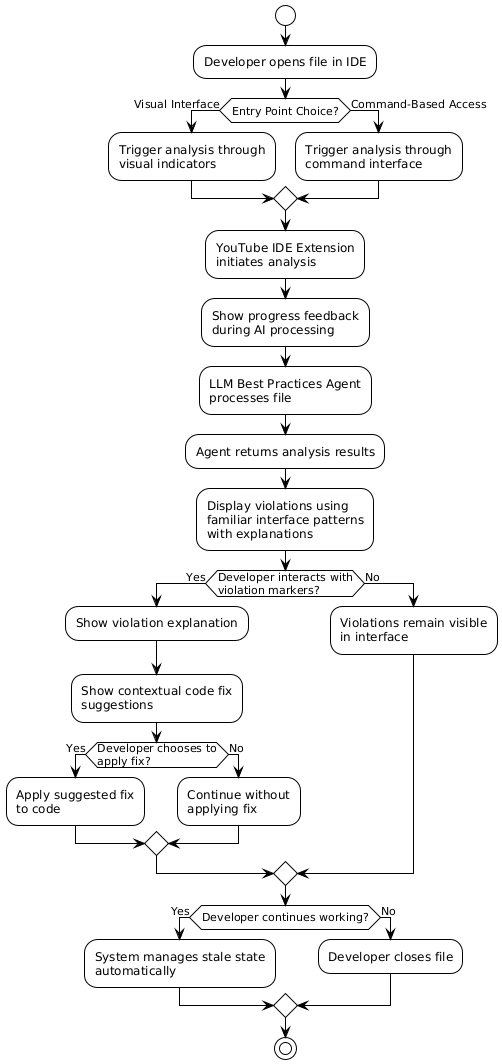
\includegraphics[scale=0.6]{images/user_flow.png}
\caption{YouTube IDE Extension User Interaction Flow: Complete developer journey from analysis trigger to fix application}
\label{fig:user_interface_flow}
\end{figure}

The flow demonstrates the core interaction pattern: developers initiate analysis through visual or command interfaces, receive progress feedback during processing, and interact with displayed violations to access explanations and optional fixes. This design ensures developers maintain control over their workflow while providing comprehensive feedback when requested.


\section{Data Models and Interfaces}

\subsection{Input/Output Specification}
The system's data models define the contracts between components, ensuring consistent communication and data exchange throughout the analysis pipeline. These interfaces establish clear boundaries between the IDE extension and the AI agent, enabling independent evolution of each component.

\paragraph{Analysis Request Format}
The YouTube IDE Extension sends analysis requests to the LLM Best Practices Agent using a minimal input format that identifies the target file for analysis. This design choice ensures that the agent can focus on its core responsibility of code analysis while maintaining security and proper workspace isolation. The request format includes the file path.

\paragraph{Analysis Response Format}
The agent returns a structured response containing the analysis results, error information, and optional metadata. The response format includes status information indicating success or failure, violation details with explanations and suggested fixes, and usage statistics for monitoring purposes. This standardized format ensures that the IDE extension can consistently process and display results regardless of the underlying analysis complexity.

\subsection{Convention Data Management}
The system's convention data model defines how YouTube framework best practices are structured, stored, and accessed throughout the analysis pipeline.

\paragraph{Convention Data Structure}
The convention data model captures best practice definitions as structured objects that support efficient programmatic access and analysis. Each convention definition includes essential metadata such as unique identifiers, descriptions, correct examples, and incorrect examples. This structure enables rapid lookup and context-specific retrieval during code analysis, with the design optimized for constant-time access patterns required by the agent's processing pipeline.

\paragraph{Storage Architecture Decision}
The system employs an in-memory storage approach using structured Python objects rather than external file-based or database storage. This design decision balances several architectural considerations:

\begin{itemize}
    \item \textbf{Data Characteristics}: Conventions are static during runtime, requiring no dynamic updates, making in-memory storage appropriate for performance-critical analysis.
    \item \textbf{Performance Requirements}: In-memory access ensures ultra-low-latency retrieval for real-time analysis, eliminating I/O overhead during agent execution.
    \item \textbf{Simplicity \& Reliability}: Structured Python objects provide type safety and eliminate parsing overhead while ensuring data integrity.
    \item \textbf{Resource Efficiency}: Conventions are loaded once at startup, minimizing runtime resource consumption and avoiding repeated file system access.
    \item \textbf{Architectural Flexibility}: The design allows future migration to external storage if multi-framework support or dynamic updates become necessary.
\end{itemize} 

\paragraph{Integration Interfaces}
The system defines minimal, versioned boundaries that keep components decoupled:

\begin{itemize}
    \item \textbf{IDE Extension Interface}: Contract between the YouTube IDE Extension and the LLM Best Practices Agent that defines the analysis request and response format, enabling independent evolution of UI and agent components.
    \item \textbf{Convention Access Interface}: Defines how the agent accesses convention definitions through in-memory lookup mechanisms, providing a stable boundary for data retrieval without external dependencies.
    \item \textbf{Monitoring Interface}: Captures usage statistics and performance metrics for system observability and evaluation purposes.
\end{itemize}


\subsection*{Conclusion}
The architecture of the LLM Best Practices Agent is defined by three central design decisions. First, the adoption of the Executable Agent paradigm ensures deterministic execution, structured tool orchestration, and predictable performance, avoiding the drawbacks of open-ended reasoning loops. Second, the hybrid parallel–sequential processing strategy balances efficiency with interpretability, allowing analyses to scale while maintaining transparency in intermediate results. Finally, the IDE extension provides a seamless developer experience, integrating feedback, explanations, and fixes directly into familiar workflows while managing state and staleness automatically. Together, these pillars create a robust, cost-efficient, and developer-friendly system for embedding AI-driven best practice enforcement into the coding environment.
%==============================================================================
\end{spacing}

\setcounter{chapter}{3}
\chapter{Implementation}
\minitoc %insert la minitoc
\graphicspath{{Chapitre4/figures/}}

%\DoPToC
%==============================================================================
\pagestyle{fancy}
\fancyhf{}
\fancyhead[R]{\bfseries\rightmark}
\fancyfoot[R]{\thepage}
\renewcommand{\headrulewidth}{0.5pt}
\renewcommand{\footrulewidth}{0pt}
\renewcommand{\chaptermark}[1]{\markboth{{\chaptername~\thechapter. #1 }}{}}
\renewcommand{\sectionmark}[1]{\markright{\thechapter.\thesection~ #1}}

\begin{spacing}{1.2}

%==============================================================================
\section*{Introduction}
This chapter presents the evaluation results that informed the final architecture choice, then details how we implemented that choice. We report what the evaluation revealed and, based on those results, what we chose and how it is realized in the system.

The chapter is structured as follows: first, we present the evaluation results and architecture decision; then, we describe the working environment and technology stack; finally, we detail the implementation of both the AI agent backend and the IDE extension frontend.

\section{Working Environment}

\subsection{Development Infrastructure}
The implementation leverages Google's internal development infrastructure, providing support for large-scale software development. This infrastructure ensures security, scalability, and integration with existing YouTube development workflows.

\subsubsection{Internal IDE}
The development environment utilizes Google's internal IDE, which provides a development experience similar to Visual Studio Code but optimized for Google's internal infrastructure and security requirements.

\subsubsection{Internal RPC Playground}
The RPC Playground is Google's internal tool for testing and debugging Remote Procedure Call (RPC) services~\cite{rpc1984}. This tool serves as a playground for sending RPC requests and was essential for developing and testing the communication protocol between the AI Agent and the YouTube IDE Extension.

\subsubsection{Google Colab}
Google Colab was used during early prototyping to iterate on prompt design, tool orchestration, and Executable Agent behaviors before production hardening. Colab provided hosted notebooks with on-demand compute (including GPUs/TPUs) and easy sharing for rapid experiments \cite{colab2017, jupyter2014}. It was part of the development environment rather than the deployed technology stack.


\subsubsection{Internal Repository Integration}
All code is stored and versioned within Google's internal repository system, enabling proper code review processes and collaboration.

\subsection{Project Management and Documentation}

\subsubsection{Internal Version Control}
The project utilizes Google's internal version control system, which provides Git-like functionality while ensuring compliance with internal security and access control requirements. Git is a fast, scalable, distributed version control system designed to handle everything from small to very large projects with speed and efficiency \cite{git2005}.


\subsubsection{Internal Code Review Platform}
Google's internal code review platform provides code review capabilities, ensuring code quality and knowledge sharing across development teams.

The code review platform includes:
\begin{itemize}
    \item \textbf{Automated Review Suggestions}: AI-powered suggestions for code improvements, best practices, and potential issues.
    \item \textbf{Collaborative Review Process}: Tools for managing review workflows, assigning reviewers, and tracking review progress.
    \item \textbf{Integration with CI/CD}: Automatic triggering of builds and tests when code changes are submitted for review~\cite{ci_cd2010}.
\end{itemize}

\subsubsection{Internal Project Management System}
The project management system provides project tracking, task management, and collaboration capabilities similar to Jira but optimized for Google's internal workflows. JIRA is a flexible issue tracking system that provides project management capabilities \cite{jira2002}.


\subsubsection{Google Docs}
Google Docs was used for authoring and reviewing design documents, leveraging the internal built-in Approvals workflow to formalize stakeholder sign-off. The review process combined live comments, suggestions, and targeted approvals to ensure traceable decisions.


These project workflows ensured fast iteration, early detection of issues, and compliance with Google's security and code quality standards.



\section{Technologies}

This section presents the concrete technologies used to implement the system. We distinguish between industry-standard tools (e.g., Python, TypeScript, JSON) and internal platforms operated within Google (e.g., YouTube DevInfra Agent Framework, internal AI platform).

\subsection{Backend Technologies (AI Agent)}

\subsubsection{Python Programming Language}
Python serves as the primary programming language for the AI agent framework implementation. Python is a high-level, interpreted programming language known for its simplicity, readability, and library ecosystem \cite{van1995python}. The language's dynamic typing and support for artificial intelligence and machine learning libraries make it suitable for AI agent development \cite{pedregosa2011scikit}.



Python's advantages for this implementation include:
\begin{itemize}
    \item \textbf{AI/ML Ecosystem}: Extensive libraries for machine learning, natural language processing, and AI development.
    \item \textbf{Asynchronous Programming}: Built-in support for asynchronous programming patterns essential for handling concurrent requests.
    \item \textbf{JSON Processing}: Native support for JSON serialization and deserialization required for API communication.
\end{itemize}

% (Colab moved under Development Infrastructure as a prototyping environment)


\subsubsection{YouTube DevInfra Agent Framework}
The implementation utilizes the YouTube DevInfra Agent Framework — the serving infrastructure designed by YouTube for YouTube Developer Infrastructure agents. It underpins all YouTube agents, providing standardized execution, deployment, and operational primitives for LLM-powered applications.

This framework was selected because it natively supports the \textit{Executable Agent} pattern and supplies built-in tool orchestration, workflow control, and production lifecycle management. Using it aligns the implementation with DevInfra standards and avoids rebuilding common agent infrastructure, allowing focus on best-practices enforcement logic.



\subsubsection{Internal AI Platform}
The system integrates with Google's internal AI platform, which hosts internal LLM models trained on Google's codebase, ensuring organization-specific knowledge and compliance with internal security requirements.


\subsubsection{LLM Libraries and Frameworks}
The internal agent framework utilizes several specialized libraries and frameworks for LLM interaction and agent development:

\begin{itemize}
    \item \textbf{LLM Interaction Libraries}: Specialized libraries for communicating with internal LLM models, monitoring token usage, and optimizing API calls.
    \item \textbf{Agent Orchestration Libraries}: Libraries that provide the Executable Agent pattern implementation, tool registration, and workflow management.
    \item \textbf{Prompt Engineering Libraries}: Frameworks for constructing, optimizing, and managing prompts.
\end{itemize}

\subsection{Frontend Technologies (IDE Extension)}

\subsubsection{TypeScript Programming Language}
TypeScript is used for the frontend development of the YouTube IDE Extension. TypeScript is a strongly typed superset of JavaScript that compiles to plain JavaScript \cite{bierman2014understanding}. The language provides static type checking, which helps prevent runtime errors and improves code maintainability in large-scale applications.

TypeScript was chosen because we are building a feature inside an existing extension implemented in TypeScript, ensuring direct compatibility and reuse. Its static typing and interfaces improve maintainability and reduce runtime errors in complex UI state and service interactions. It also integrates seamlessly with VS Code API and other development environments.


\subsubsection{VS Code Extension API}
The system integrates with Visual Studio Code through its Extension API. Visual Studio Code is a source-code editor developed by Microsoft, built on the Electron framework \cite{castor2016visual}. The VS Code Extension API provides capabilities for extending the editor's functionality.

Given that the internal IDE is VS Code–like, adopting the VS Code Extension API is the natural choice: it is natively supported within the environment (requiring no additional infrastructure), exposes the command, user‑interface, and configuration interfaces required by the best‑practices enforcement feature, and ensures compatibility with the existing extension ecosystem. In practice, the API provides the integration points necessary to implement the designed interaction flow without introducing custom runtime scaffolding.


\section{Realization}

The realization phase translates architectural decisions into a concrete implementation of the system. 
It consists of two primary components: (1) the \textbf{AI Agent backend}, responsible for code analysis 
and violation handling, and (2) the \textbf{IDE Extension frontend}, responsible for developer interaction. 
This section first discusses the evaluation results that informed our architectural choice, then presents 
the detailed implementation of the agent and its integration with the IDE extension.

\subsection{Agent Realization}

\subsubsection{Evaluation Results and Architecture Decision}
To determine the most suitable agent design, we evaluated three candidate architectures: the Parallel Executable, 
Sequential Executable, and ReAct Agent. These were assessed against 12 representative test cases covering 
a range of violation patterns and code complexities.  

For a simple single-violation file (TC8\_PROPS\_MISSING\_EXPORT), the results are shown in 
Table~\ref{tab:single_violation_performance_ch4}. Parallel outperformed Sequential by $\sim$33\% in latency, 
while both were vastly more efficient than ReAct in token usage.

\begin{table}[H]
\centering
\caption{Single-Violation File Performance Comparison}
\label{tab:single_violation_performance_ch4}
\footnotesize
\begin{tabular}{|l|c|c|c|}
\hline 
\textbf{Architecture} & \textbf{Latency} & \textbf{Input Tokens} & \textbf{Output Tokens} \\
\hline 
Parallel Executable & 4.1s & 5,157 & 331 \\
\hline
Sequential Executable & 6.1s & 5,157 & 331 \\
\hline
ReAct Agent & 15.3s & 37,989 & 1,523 \\
\hline
\end{tabular}
\end{table}

Scaling to the full evaluation suite (Figures~\ref{fig:latency_comparison_ch4}--\ref{fig:accuracy_comparison_ch4}) 
revealed deeper trade-offs. Parallel maintained faster throughput but suffered reliability issues such as 
\texttt{OverLimitException} and \texttt{DEADLINE\_EXCEEDED}. Sequential was slower but fully reliable with identical 
accuracy ($\sim$91.7\%). ReAct proved infeasible due to extreme token consumption and lower accuracy.

\begin{figure}[H]
\centering
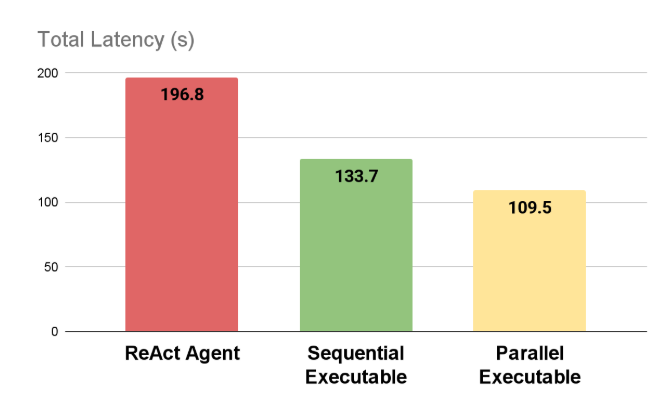
\includegraphics[scale=0.5]{images/latency.png}
\caption{Latency Performance Across 12 Test Cases}
\label{fig:latency_comparison_ch4}
\end{figure}

\begin{figure}[H]
\centering
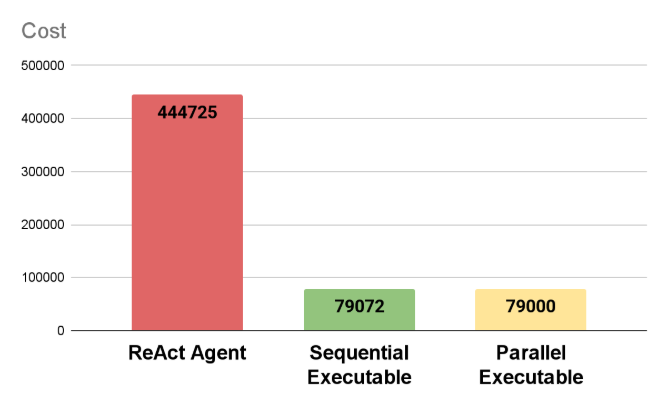
\includegraphics[scale=0.5]{images/cost.png}
\caption{Cost Analysis Across 12 Test Cases}
\label{fig:cost_comparison_ch4}
\end{figure}

\begin{figure}[H]
\centering
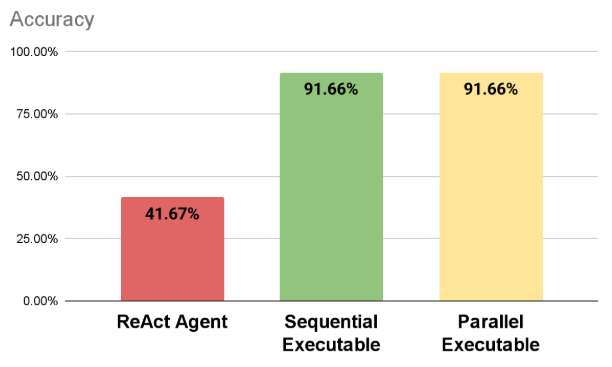
\includegraphics[scale=0.5]{images/accuracy.png}
\caption{Accuracy Performance Across 12 Test Cases}
\label{fig:accuracy_comparison_ch4}
\end{figure}

From these results, the final decision was to adopt a \textbf{Parallel Executable architecture with concurrency limiting}. 
This preserves most of the performance advantage of Parallel while ensuring reliability through semaphore-based 
concurrency control, preventing resource saturation. This hybrid approach combines determinism, throughput, and robustness, 
making it suitable for production use in developer IDEs.

\subsubsection{Agent Implementation Overview}
The AI Agent implements the chosen architecture using Python and integrates with Google’s internal AI platform 
hosting Gemini-based LLMs. The design is class-based and modular, ensuring extensibility, observability, and testability.  
The agent exposes a single \texttt{execute()} entry point, orchestrating a pipeline of specialized tools that handle 
file reading, analysis, explanation generation, fix generation, and result consolidation.

\paragraph{Configuration and Initialization}
At startup, the agent performs several critical setup tasks:
\begin{itemize}
    \item \textbf{Model Selection:} Configured to use the latest Gemini-based model trained on internal Google code.
    \item \textbf{Convention Loading:} Best practices are retrieved from repository-stored JSON files and cached in memory.
    \item \textbf{Tool Registration:} The five specialized tools are instantiated and registered into a deterministic workflow.
\end{itemize}

\paragraph{Implementation Structure}
The implementation follows a layered orchestration pattern:
\begin{itemize}
    \item A central agent class orchestrates the pipeline via dependency-injected tools.
    \item Each tool is encapsulated as a class with clear \texttt{run()} contracts and typed inputs/outputs.
    \item Metrics and token usage are logged per tool, enabling fine-grained observability.
    \item Separation of concerns allows tools to be replaced or extended without modifying orchestration logic.
\end{itemize}

\subsubsection{Core Tools Implementation}
The agent implements five specialized tools, each corresponding to one stage of the analysis pipeline. Tools are designed as independent classes that expose a public \texttt{run()} method, which enforces a clear input/output contract and raises typed errors when failures occur. This contract-based design makes the system modular, testable, and resilient to partial failures.

\paragraph{ReadFileFromWorkspace Tool}
\textbf{Contract:} input = file path; output = file content (string).  
The ReadFileFromWorkspace tool is responsible for retrieving the contents of the developer’s source file. Implementation details include:
\begin{itemize}
    \item \textbf{File system access:} Uses Python’s built-in file handling with UTF-8 as the default encoding, while detecting and recovering from alternative encodings.
    \item \textbf{Error handling:} Raises typed errors such as \texttt{FileNotFoundError}, \texttt{PermissionDeniedError}, and \texttt{EncodingError}. These errors are logged and surfaced to the developer in structured form.
    \item \textbf{Robustness:} Handles large files by streaming content, ensuring memory efficiency.
\end{itemize}

\paragraph{CodeAnalysisTool}
\textbf{Contract:} input = file content; output = list of base violations.  
This tool forms the analysis core of the system. It detects framework violations by orchestrating LLM queries enriched with contextual information.
\begin{itemize}
    \item \textbf{Prompt construction:} Implements a template system with slots for file type, code snippet, and dynamically filtered convention definitions.
    \item \textbf{Context injection:} Selects relevant conventions from the cache and injects them into the prompt to guide the model.
    \item \textbf{Response parsing:} Uses strict JSON schema validation with recovery mechanisms for malformed LLM responses.
    \item \textbf{Performance optimizations:} Employs caching of templates and convention definitions, reducing repeated token usage and lowering latency.
\end{itemize}

\paragraph{ViolationExplanationTool}
\textbf{Contract:} input = base violation; output = natural-language explanation.  
The ViolationExplanationTool generates educational explanations that help developers understand not only what the violation is, but why it matters.
\begin{itemize}
    \item \textbf{Contextualization:} Pulls in violation metadata (rule violated, line number, code snippet) to ground explanations in concrete evidence.
    \item \textbf{Generation style:} Prompts the LLM to balance technical accuracy with readability, avoiding overly generic statements.
    \item \textbf{Implementation detail:} Each explanation is post-processed for clarity, removing redundant phrasing and enforcing concise output.
\end{itemize}

\paragraph{CodeFixTool}
\textbf{Contract:} input = violation + explanation; output = code fix (annotated snippet).  
This tool provides actionable, safe, and educational fixes.
\begin{itemize}
    \item \textbf{Safety:} Fixes are constrained to local code changes, avoiding edits that break APIs or dependencies.
    \item \textbf{Self-containment:} Ensures that each fix can be applied without requiring modifications in other files.
    \item \textbf{Contextual adaptation:} Uses file content and violation metadata to adapt fixes to the surrounding code style.
    \item \textbf{Educational emphasis:} Each fix includes explanatory comments describing why the change is required.
    \item \textbf{Error handling:} Raises a \texttt{FixGenerationError} if the LLM output cannot be parsed or validated as compilable code.
\end{itemize}

\paragraph{Finish Tool}
\textbf{Contract:} input = violations + explanations + fixes; output = structured response for IDE extension.  
The Finish Tool acts as the consolidation component, producing a structured JSON-like response that the IDE extension can directly render.
\begin{itemize}
    \item \textbf{Aggregation:} Combines violations, explanations, and fixes into a unified structure keyed by violation ID.
    \item \textbf{Deduplication:} Identifies overlapping or redundant violations and merges them to reduce noise.
    \item \textbf{Validation:} Ensures schema compliance so that the IDE can reliably parse and render results.
    \item \textbf{Formatting:} Applies consistent formatting (line numbers, code blocks, explanations) to improve readability in the UI.
\end{itemize}

\noindent Collectively, these tools form a deterministic pipeline coordinated by the agent’s \texttt{execute()} method. Each tool adheres to explicit contracts, which improves modularity, observability (per-tool token usage is logged), and long-term maintainability.


\subsubsection{Processing Workflow}
The hybrid strategy is realized in three stages:
\begin{enumerate}
    \item \textbf{Sequential Preprocessing:} Full file content is read and all violations are identified.
    \item \textbf{Parallel Processing:} Explanation and fix generation tasks are executed concurrently with semaphore-based 
    limits on in-flight LLM calls.
    \item \textbf{Result Consolidation:} Outputs are aggregated, validated, and prepared for the IDE extension.
\end{enumerate}

Figure~\ref{fig:agent_activity} illustrates this workflow.

\begin{figure}[H]
    \centering
    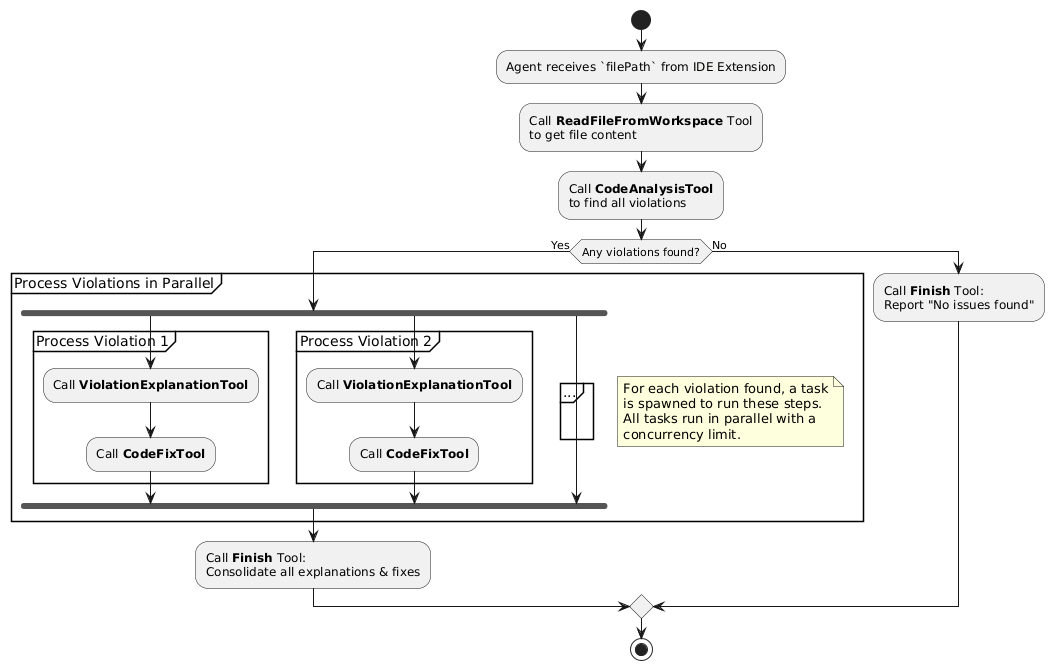
\includegraphics[scale=0.5]{images/activity_diagram.png}
    \caption{Agent Processing Activity Diagram}
    \label{fig:agent_activity}
\end{figure}

\subsubsection{Resilience and Error Handling}
The system ensures graceful degradation under failures:
\begin{itemize}
    \item Independent processing of violations isolates failures to individual tasks.
    \item Retry with exponential backoff mitigates transient network or LLM errors.
    \item Typed error classes facilitate debugging and developer support.
    \item Partial results are preserved, ensuring developers always receive usable feedback.
\end{itemize}

\subsubsection{Convention Data Management}
The convention data management system implements loading, caching, and retrieval mechanisms for YouTube framework best practices. The conventions are stored as Python objects in an array, each containing a unique identifier, description, correct example, and incorrect example. For efficient runtime access, the system constructs an in-memory map keyed by convention ID, allowing the agent tools to retrieve only the relevant convention on demand. 

\paragraph{Loading and Initialization}
At startup, all convention objects are loaded into memory from the Python array. A dictionary (map) is created with convention IDs as keys and convention objects as values, providing constant-time access for subsequent tool invocations.

\paragraph{Memory Caching and Access}
This in-memory caching strategy ensures low-latency access during code analysis:

\begin{itemize}
    \item \textbf{Efficient Lookup}: Tools retrieve conventions by ID from the map, avoiding iteration over the full array.
    \item \textbf{Dynamic Selection}: Only conventions relevant to the current file type and analysis context are queried, minimizing unnecessary data processing.
    \item \textbf{Lightweight and Fast}: The cache resides entirely in memory, requiring no external services, and supports rapid retrieval during concurrent tool executions.
\end{itemize}

\subsection{Extension Integration}

\subsubsection{Extension Architecture}
The IDE Extension implements a layered architecture that integrates with the overall system through three distinct layers: the Extension layer containing user-facing components, a Proxy layer for authentication and request routing, and the Backend layer hosting AI agent services.

\begin{figure}[H]
    \centering
    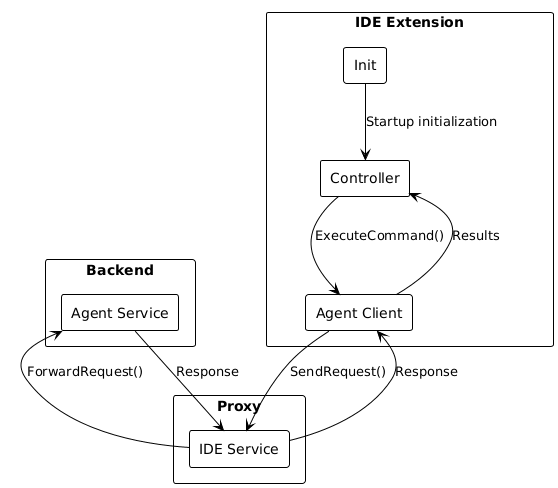
\includegraphics[scale=0.6]{Images/extension_integration.png}
    \caption{System Architecture: IDE Extension, Proxy, and Backend Communication Flow}
    \label{fig:high_level_frontend_architecture}
\end{figure}

The architecture follows a clear request-response pattern where user interactions trigger analysis requests that flow through the IDE Service proxy for authentication and authorization, then to the Agent Service in the backend for processing. Responses follow the same path in reverse, ensuring secure and authenticated communication throughout the entire pipeline while maintaining clear separation of responsibilities between layers.

\paragraph{Extension Components}
The extension's internal architecture consists of three core components that work together to provide seamless integration with the development environment, as illustrated in Figure~\ref{fig:high_level_frontend_architecture}.

\textbf{Init Component}: Handles extension initialization, reading user settings, registering commands and editor actions, and performing health checks. The component ensures proper setup of all dependencies.

\textbf{Controller}: Centralizes all UI-related state and orchestrates interactions between components. The Controller processes commands, manages notifications, routes analysis results, renders diagnostics and hover-based suggestions, and coordinates stale-state transitions to ensure consistent behavior across all entry points.

\textbf{AgentClient}: Manages communication with the backend services through the proxy layer. The component handles request formatting, implements retry logic with exponential backoff, manages timeouts, and processes responses from the AI agent.

\subsubsection{User Interaction}
The feature is controlled through a dedicated \textbf{user setting}. This setting appears as a simple checkbox: when enabled, the feature becomes available in the IDE; when disabled, it is entirely hidden from the interface. This ensures that developers can opt in seamlessly without cluttering the environment for those who do not use the feature.

The primary entry point for triggering analysis is an \textbf{Editor Action} integrated into the file title bar (Figure~\ref{fig:editor_action_implementation}). This placement ensures high visibility and aligns naturally with the developer’s workflow when working on individual files.

\begin{figure}[H]
    \centering
    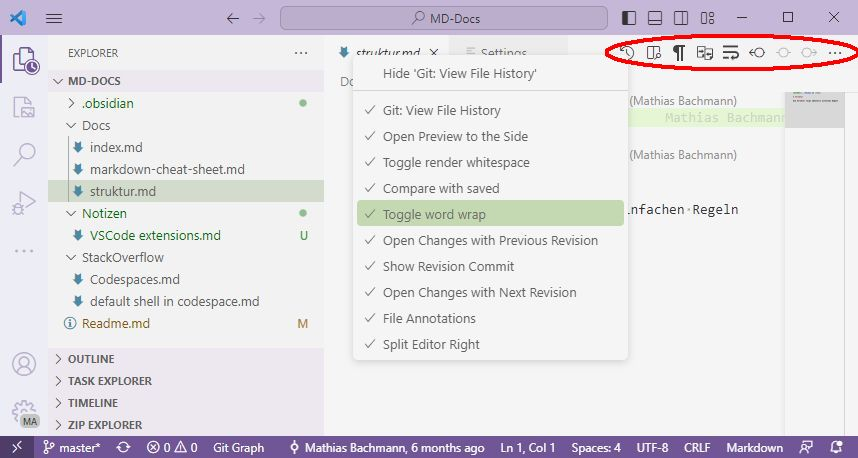
\includegraphics[scale=0.4]{Images/editor_actions.jpg}
    \caption{VS Code Interface: Editor Actions (Illustrative).}
    \label{fig:editor_action_implementation}
\end{figure}

An additional entry point is provided through the \textbf{Command Palette}, which can be invoked using \texttt{Ctrl+Shift+P} (or \texttt{Cmd+Shift+P} on macOS). This pathway makes the feature equally accessible to developers who prefer keyboard-driven workflows and ensures discoverability for new users exploring available commands (Figure~\ref{fig:command_palette_example}).

\begin{figure}[H]
    \centering
    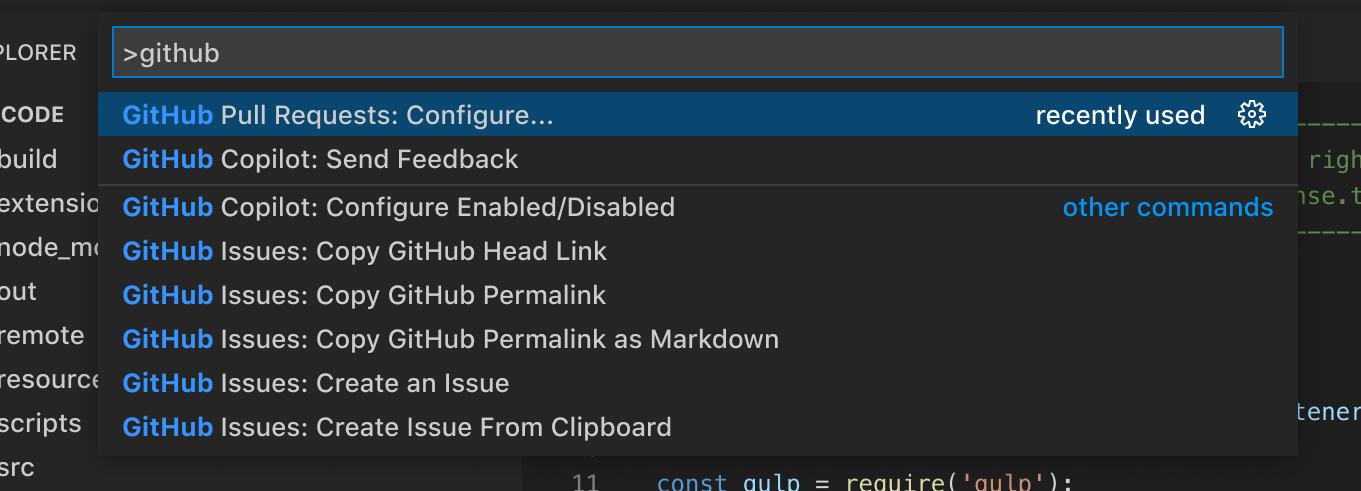
\includegraphics[scale=0.5]{Images/command_palette.png}
    \caption{VS Code Command Palette (Illustrative).}
    \label{fig:command_palette_example}
\end{figure}


Once analysis is triggered, the extension provides immediate feedback via \textbf{VS Code notifications} (Figure~\ref{fig:notification_example}). These notifications confirm that a request has been received, update progress, and display clear error messages if issues occur. This ensures transparent communication throughout the request lifecycle.

\begin{figure}[H]
    \centering
    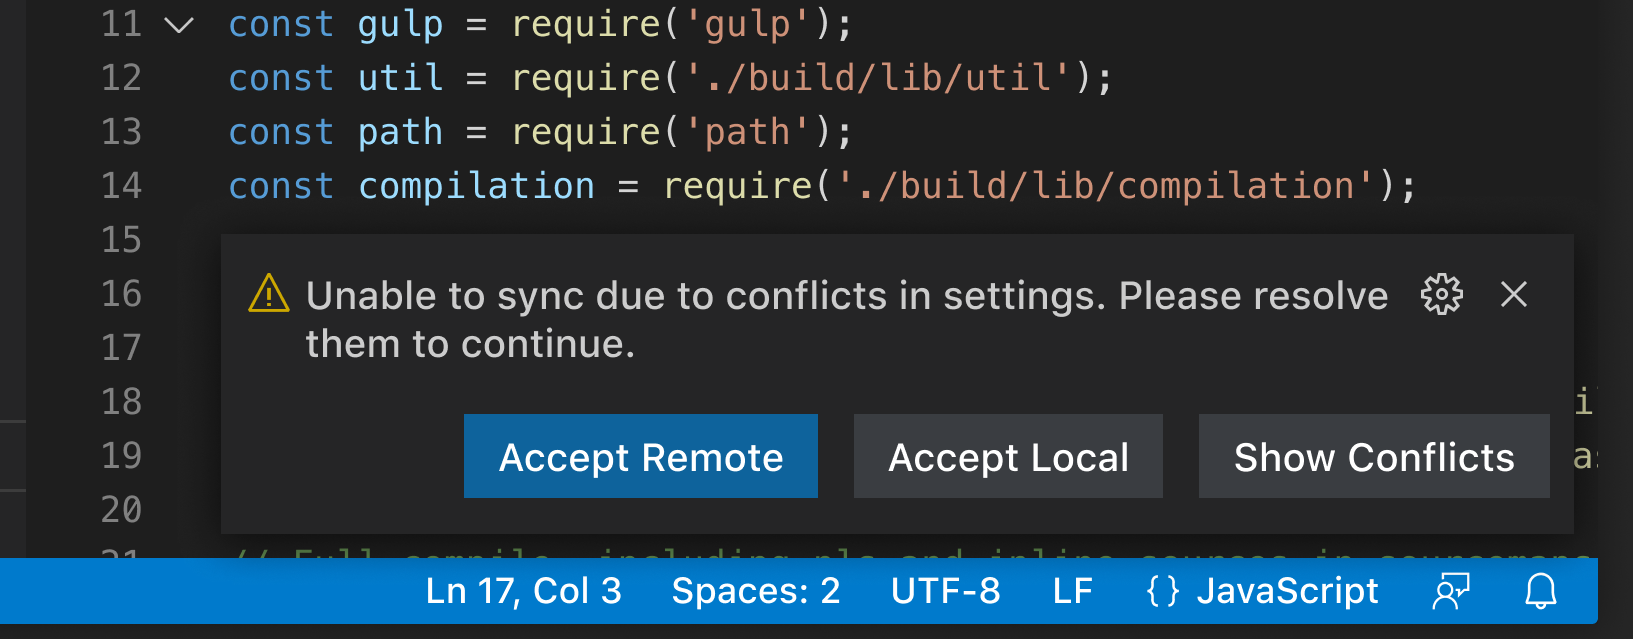
\includegraphics[scale=0.8]{Images/vscode_notification.png}
    \caption{VS Code Notification Interface (Illustrative).}
    \label{fig:notification_example}
\end{figure}

The results of the analysis are surfaced through VS Code’s native \textbf{diagnostic system}. Violations appear in the \textbf{Problems panel} and are underlined directly in the editor, marking the exact range of code that violates a best practice (Figure~\ref{fig:diagnostics_example}). Hovering over the highlighted code reveals the diagnostic explanation, helping developers quickly understand the issue in context.

\begin{figure}[H]
    \centering
    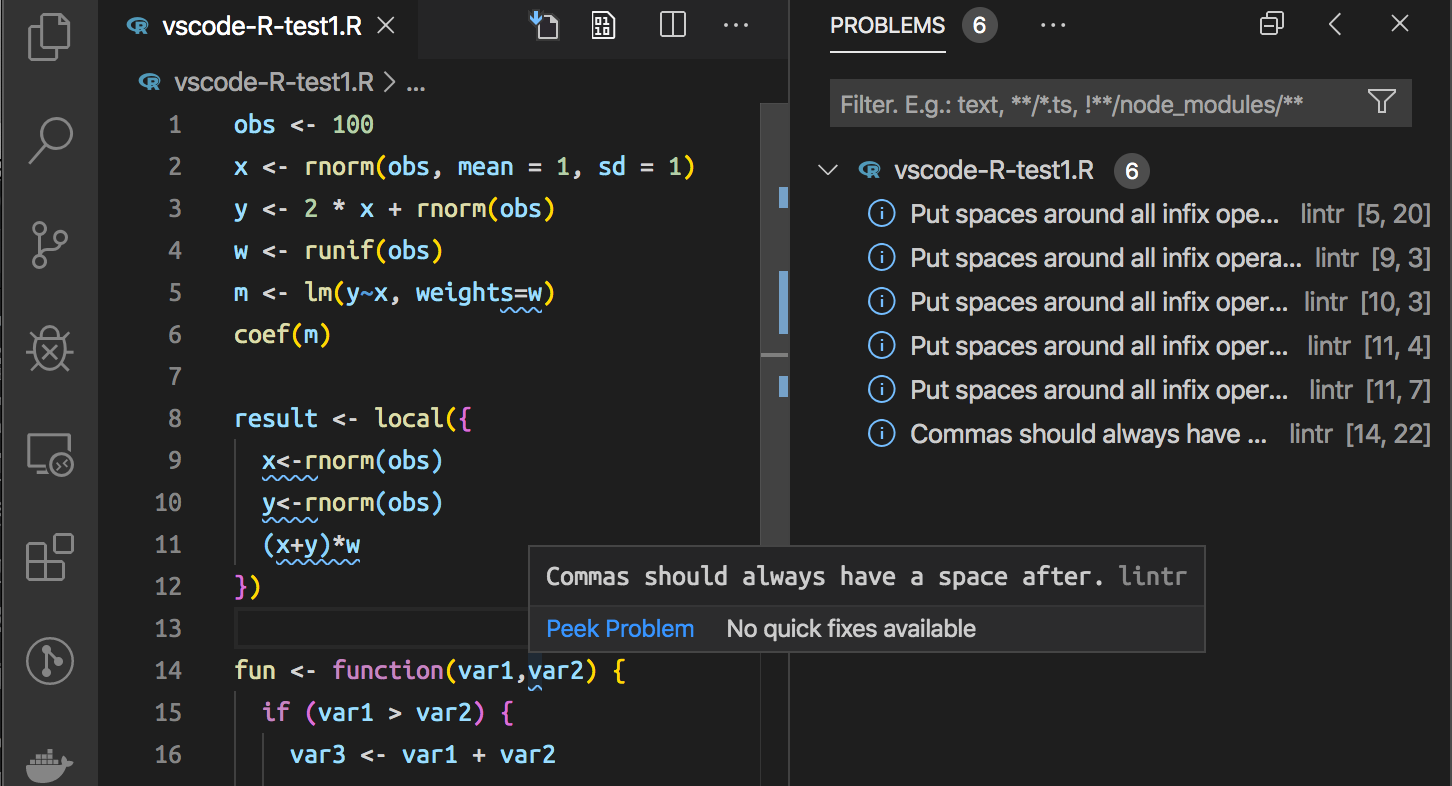
\includegraphics[scale=0.4]{Images/vscode_diagnostics.png}
    \caption{VS Code Diagnostics Interface (Illustrative).}
    \label{fig:diagnostics_example}
\end{figure}

For more detailed guidance, an integrated \textbf{hover provider} presents formatted fix suggestions directly within the editor. This approach allows fixes to be displayed with proper syntax highlighting and inline code snippets, offering a clear and actionable path to resolution without leaving the development workflow.

\subsubsection{Stale Diagnostics Handling}
One of the most challenging aspects of IDE integration is maintaining diagnostic accuracy as developers continuously modify their code. The extension implements a sophisticated two-tiered system that balances immediate responsiveness with accurate analysis results.

\paragraph{The Challenge}
Traditional diagnostic systems struggle with code that changes rapidly, often displaying outdated information that confuses developers and reduces trust in the tool. The challenge is to provide immediate visual feedback while ensuring that diagnostics remain accurate and relevant to the current code state.

\paragraph{Two-Tiered Solution}  
The extension handles stale diagnostics using a two-tiered approach that separates immediate responsiveness from precise re-anchoring:  

\textbf{Tier 1 - Instant Adjustment}: Provides immediate feedback on every keystroke. Diagnostics are shifted based on simple text edits and marked as [Outdated] if the flagged code itself is edited. This ensures high \textbf{responsiveness} without impacting performance.  

\textbf{Tier 2 - Debounced Re-anchoring}: Activates after a 1-second pause in typing to improve diagnostic \textbf{accuracy}. The process involves:  
\begin{enumerate}
    \item \textbf{Fingerprint}: Creates a contextual hash from the code and its surrounding context to identify exact matches.  
    \item \textbf{Scan with Regex}: Finds all possible text matches across the document.  
    \item \textbf{Re-anchor}: Moves the diagnostic to the correct new location based on the highest match score.  
\end{enumerate}  
This two-tiered strategy balances responsiveness with accuracy, ensuring developers receive timely feedback while maintaining the integrity of diagnostics even during active code editing.


\begin{figure}[H]
    \centering
    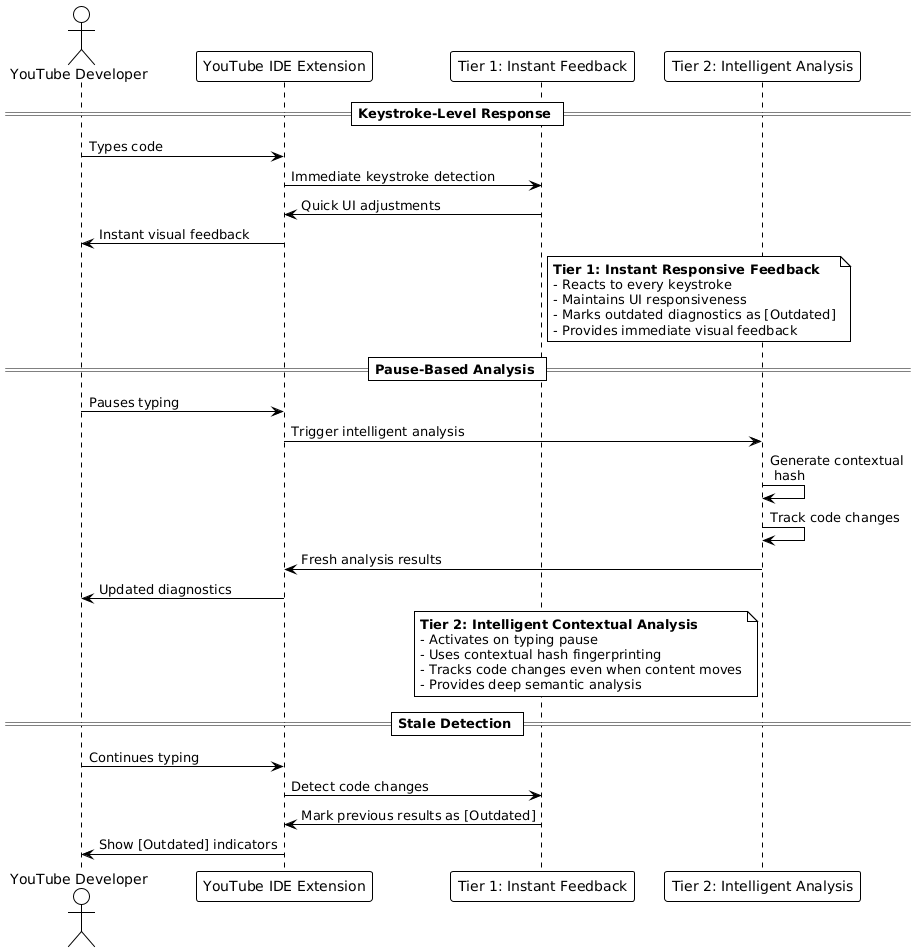
\includegraphics[scale=0.55]{Images/stale_diagnostics.png}
    \caption{Stale Diagnostics Handling: Two-Tiered System (Illustrative)}
    \label{fig:stale_diagnostics_method}
\end{figure}

This approach ensures that developers receive immediate visual feedback while maintaining diagnostic accuracy through intelligent analysis timing and state management, representing a significant technical contribution to IDE integration challenges.

\subsubsection{Resilience and Communication}
The extension implements comprehensive error handling and resilience mechanisms to ensure reliable operation in production environments. The communication system uses internal RPC infrastructure with JSON payloads for debugging and cross-language compatibility.

Error handling follows fault-tolerant design principles with multi-level error isolation, ensuring that failures in one component do not cascade to others. The system implements specific error types for different failure scenarios, including network communication errors, service unavailability, and timeout errors, with detailed error information and suggested recovery actions.

Retry mechanisms with exponential backoff and bounded attempts ensure operation under transient failure conditions, while timeout management prevents indefinite waiting periods and maintains responsive user experience. The implementation includes request validation and response parsing to prevent communication errors and ensure data integrity throughout the analysis pipeline.


\section*{Conclusion}
This chapter presented the evaluation results, the resulting architecture decision (Parallel Executable with concurrency limiting), and the complete implementation: environment, technologies, and realization across backend and IDE. The system is production-oriented, balancing speed with stability and cost.

%==============================================================================
\end{spacing}
% Chapter 5 removed after splitting its content across Chapters 3 and 4

\backmatter
\pagestyle{fancy}
\fancyhf{}
\renewcommand{\chaptermark}[1]{\markboth{Conclusion and Perspectives}{}}
\fancyhead[R]{Conclusion and Perspectives}
\fancyfoot[R]{\thepage}
\renewcommand{\headrulewidth}{0.5pt}
\renewcommand{\footrulewidth}{0pt}
\chapter{Conclusion and Perspectives}
%==============================================================================
\pagestyle{fancy}
\fancyhf{}
\fancyhead[R]{\bfseries\rightmark}
\fancyfoot[R]{\thepage}
\renewcommand{\headrulewidth}{0.5pt}
\renewcommand{\footrulewidth}{0pt}
\renewcommand{\chaptermark}[1]{\markboth{\MakeUppercase{\chaptername~\thechapter. #1 }}{}}
\renewcommand{\sectionmark}[1]{\markright{\thechapter.\thesection~ #1}}

\begin{spacing}{1.2}
%==============================================================================

C'est l'une des parties les plus importantes et pourtant les plus négligées 
du rapport. Ce qu'on \underline{ne veut pas voir} ici, c'est combien ce stage vous a été bénéfique, comment il vous a appris à vous intégrer, à connaître le monde du travail, etc.\\
Franchement, personne n'en a rien à faire, du moins dans cette partie. Pour cela, vous 
avez les remerciements et les dédicaces, vous pourrez vous y exprimer à souhait.\\
La conclusion, c'est très simple : c'est d'abord le résumé de ce que vous avez raconté
dans le rapport : vous reprenez votre contribution, en y ajoutant ici les outils que vous 
avez utilisé, votre manière de procéder. Vous pouvez même mettre les difficultés
rencontrées. En deuxième lieu, on y met les perspectives du travail : ce qu'on pourrait 
ajouter à votre application, comment on pourrait l'améliorer.

%==============================================================================
\end{spacing}

\bibliographystyle{Biblio/unsrt_modif} 
\singlespacing
\renewcommand{\bibname}{References}

\bibliography{Biblio/aesm_edspia}

\onehalfspacing

\appendix
\setcounter{figure}{0} 
\setcounter{table}{0}
\setcounter{footnote}{0}
\setcounter{equation}{0}
\pagestyle{fancy}
\fancyhf{}
\renewcommand{\chaptermark}[1]{\markboth{\MakeUppercase{#1 }}{}}
\renewcommand{\sectionmark}[1]{\markright{\thesection~ #1}}
\fancyhead[RO]{\bfseries\rightmark}
\fancyhead[LE]{\bfseries\leftmark}
\fancyfoot[RO]{\thepage}
\fancyfoot[LE]{\thepage}
\renewcommand{\headrulewidth}{0.5pt}
\renewcommand{\footrulewidth}{0pt}

\makeatletter
\renewcommand\thefigure{A.\arabic{figure}}
\renewcommand\thetable{A.\arabic{table}} 
\makeatother

\chapter{Appendix : Miscellaneous remarks}
\graphicspath{{Annexe1/figures/}}
%==========================================================================

%    Annexe

%===========================================================================
\begin{itemize}
\item Un rapport doit toujours être bien numéroté;
\item De préférence, ne pas utiliser plus que deux couleurs, ni un caractère fantaisiste; 
\item Essayer de toujours garder votre rapport sobre et professionnel; 
\item Ne jamais utiliser de je ni de on, mais toujours le nous (même si tu as tout fait tout seul); 
\item Si on n'a pas de paragraphe 1.2, ne pas mettre de 1.1;
\item TOUJOURS, TOUJOURS faire relire votre rapport à quelqu'un d'autre (de préférence qui n'est pas du domaine) pour vous corriger les fautes d'orthographe et de français;
\item Toujours valoriser votre travail : votre contribution doit être bien claire et mise en évidence; 
\item Dans chaque chapitre, on doit trouver une introduction et une conclusion;
\item Ayez toujours un fil conducteur dans votre rapport. Il faut que le lecteur suive un raisonnement bien clair, et trouve la relation entre les différentes parties;
\item Il faut toujours que les abréviations soient définies au moins la première fois où elles sont utilisées. Si vous en avez beaucoup, utilisez un glossaire.
\item Vous avez tendance, en décrivant  l'environnement matériel, à parler de votre ordinateur, sur lequel vous avez développé : ceci est inutile. Dans cette partie, on ne cite que le matériel qui a une influence sur votre application. Que vous l'ayez développé sur Windows Vista ou sur Ubuntu n'a aucune importance;
\item Ne jamais mettre de titres en fin de page; 
\item Essayer toujours d'utiliser des termes français, et éviter l'anglicisme. Si certains termes  sont plus connus en  anglais, donner leur équivalent en français la première fois que vous les utilisez, puis utilisez le mot anglais, mais en italique;
\item Éviter les phrases trop longues : clair et concis, c'est la règle générale !\\

\newpage

\textbf{Rappelez vous que votre rapport est le visage de votre travail : un mauvais rapport peut éclipser de l'excellent travail. Alors prêtez-y l'attention nécessaire.}

 
\begin{figure}[!ht]\centering

\includegraphics[scale=0.5]{ingenieur.jpg}
\end{figure}
\end{itemize}



% Multilingual Abstracts Page
\fancyhead[R]{Multilingual Abstracts}
\thispagestyle{empty}
\begingroup
\singlespacing
\small
\setlength{\parskip}{3pt}
\setlength{\parindent}{0pt}
\enlargethispage{2\baselineskip}

% Arabic title and abstract (fully Arabic title)
\begin{otherlanguage}{arabic}
\section*{فرض أفضل الممارسات مع تكامل نموذج اللغة الكبير وبيئة التطوير المتكاملة}
أُنجز هذا المشروع في شركة جوجل زيورخ ضمن متطلبات الدبلوم الوطني للهندسة في هندسة البرمجيات. يدرس دمج الذكاء الاصطناعي التوليدي في تطوير البرمجيات عبر وكيل يعتمد على نموذج اللغة الكبير (\textLR{LLM}) داخل بيئة التطوير المتكاملة (\textLR{IDE}).

يُحلّل الوكيل الشيفرة لاكتشاف انتهاكات معقّدة قد تغفلها أدوات التحليل الثابت، ويُنتج شروحات واضحة واقتراحات عملية تساعد مطوري يوتيوب على رفع جودة الشيفرة والالتزام بالممارسات الفضلى. وباندماجه في سير العمل عن طريق إضافة للبيئة، يعزّز الإنتاجية ويقلّل الديون التقنية دون تعطيل تجربة التطوير.

\textbf{الكلمات المفتاحية: هندسة برمجيات، ذكاء اصطناعي توليدي، تكامل \textLR{IDE}، جودة الشيفرة، إنتاجية المطوّرين}
\end{otherlanguage}

\vspace{0.5cm}

% French title: Project title in French
\section*{Application des meilleures pratiques avec l'intégration LLM-IDE}
Ce projet, réalisé chez Google Zurich, intègre un agent basé sur un LLM au sein d'un IDE interne pour soutenir le développement logiciel.

L'agent analyse le code, fournit des explications claires et des suggestions actionnables, et s'intègre au flux de travail par une extension IDE. Il aide les contributeurs YouTube à maintenir une haute qualité de code et à réduire la dette technique sans perturber l'activité.

\textbf{Mots-clés : Génie logiciel, IA générative, Intégration IDE, Qualité du code, Productivité}

\vspace{0.5cm}

% English title: Project title in English
\section*{Enforcing Best Practices with LLM-IDE Integration}
This project, conducted at Google Zurich, embeds an LLM-powered agent inside an internal IDE to support software development.

The agent analyzes code to detect complex violations missed by traditional static tools, producing clear explanations and actionable fixes. Integrated via an IDE extension, it boosts productivity and reduces technical debt without disrupting the developer workflow.

\textbf{Keywords: Software Engineering, Generative AI, IDE Integration, Code Quality, Productivity}

\endgroup



\end{document}